\chapter{Foundations}\label{chapFoundations}

In this chapter the fundamentals of \gls{ModelTransformationByExample}, \glspl{ModelToModelTransformation}, \glspl{SwarmIntelligentAlgorithm} and \glspl{EvolutionaryAlgorithm} are presented to refine the requirements. The general goal is to solve \glspl{ModelToModelTransformation} using meta-heuristic optimization algorithms. Figure \ref{figProblemDomainOverview} presents an overview of the problem domain. 

\begin{figure}[htb]
	\centering
	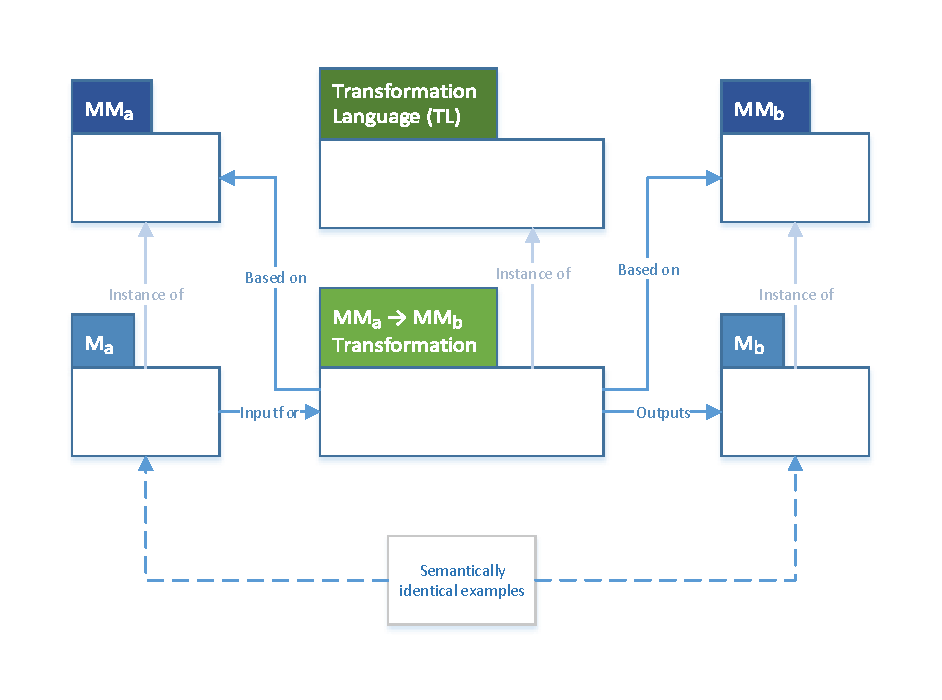
\includegraphics[scale=0.8, trim=0cm 1cm 0cm 1cm, clip=true]{Images/ProblemDomainOverview.pdf} 
	\caption{Problem domain overview - a ``MM$_a$ $\rightarrow$ MM$_b$ Transformation" has to be generated by using semantically identical input/output pairs}
	\label{figProblemDomainOverview}
\end{figure}

According to the general \gls{ModelTransformationByExample} methodology, there are two \glspl{MetaModel} MM$_a$ and MM$_b$. The task of the algorithm is to transform instances of the former into instances of the latter by performing a ``MM$_a$ $\rightarrow$ MM$_b$ Transformation". This transformation needs not be defined explicitly depending on the definition of \gls{ModelTransformationByExample}. In order to guide the algorithm, it must be able to rate a \gls{CandidateSolution}. Hence, one or more instances M$_a$ of MM$_a$ with their expected output M$_b$ conforming to MM$_b$ have to be provided. Also more information can be added as a guidance, depending on the used \gls{ModelTransformationByExample} definition. For example, details about the mapping from M$_a$ to M$_b$. This high level problem statement is refined in this chapter by answering the following questions:

\begin{itemize}
	\item What is state-of-the-art in \gls{ModelTransformationByExample}? What is the definition of \gls{ModelTransformationByExample} used in this thesis (see section \ref{secRelatedWork})? 
	\item What is a \gls{ModelToModelTransformation} given the chosen definition of \gls{ModelTransformationByExample} (see section \ref{secModelToModelTransformations})? 
	\item What renders \glspl{ModelToModelTransformation} simple or complex? What is a simple starting point for the algorithm design and development? How could the complexity be increased (see section \ref{secModelToModelTransformations})? 
	\item What are the characteristics of meta-heuristic optimization algorithms from the field of \glspl{SwarmIntelligentAlgorithm} and \glspl{EvolutionaryAlgorithm} (see section \ref{secAlgorithms})? 
	\item How can the algorithms be mapped to \gls{ModelTransformationByExample} (see section \ref{secAlgorithms})? 
\end{itemize}

%2.1 Related Work
%In order to automatically generate such ``MM$_a$ $\rightarrow$ MM$_b$ Transformations" it is at first necessary to define a more concrete goal. The first section \ref{secRelatedWork} provides an insight into existing approaches in the field of \gls{ModelTransformationByExample}. It points out the open research issues and highlights the ones that are the focus of this thesis. 

%2.2 Model-to-Model Transformations
%Transformations can have infinite different variations, which makes it difficult to find a starting point when automating those. Section \ref{secModelToModelTransformations} is therefore focusing on the identification of \glspl{ModelToModelTransformation} building-blocks.

%Therefore, at first an overview of existing \glspl{TransformationLanguage} and tools is being provided in in \ref{secExistingModelTransformationLanguagesAndTools}. Ensuring a systematic approach the idea is to identify and\/ or create definitions of a \gls{Model} and a \gls{ModelToModelTransformation} in \ref{secModelToModelTransformations} which will serve as a guideline in the universe of possible transformations. With these CMMTP at hand two kinds of examples, one for each \gls{Model} type structural and behavioral, should be created in the next chapter \ref{chapM2MScenarios} to show the actual application relevance of those for the MDD domain and at the same time provide MM$_a$ and MM$_b$ \glspl{Model} which are required to drive the prototype realization. 

%2.3 Algorithms
%In order to be able to automate \glspl{ModelToModelTransformation} a set of possible meta-heuristic optimization algorithms from the field of \glspl{SwarmIntelligentAlgorithm} and \glspl{EvolutionaryAlgorithm} are presented in section \ref{secAlgorithms}. %Those are being considered when deciding for the solution approach.

%2.4 Basic Alogrithmic Solution Approach
%Using all this information, a first draft of the algorithmic approach is being defined in section \ref{secAlgorithmicApproach}. 

%While this will already be a sound foundation it is not enough to follow the desired iterative approach yet. Therefore, an extensible example is required which will have a simple initial setup and can be extended towards a more complicated one. To define what is actually ``simple" and ``complex" a rough idea of the algorithm is needed which will be provided in  preceded by a general conceptual overview of the underlying techniques in \ref{secAlgorithms}. 

%As pointed out in \ref{figProblemDomainOverview} the ``MM$_a$ $\rightarrow$ MM$_b$ Transformation" is based on a TL which therefore must be used by the algorithm to create valid transformations. Since it is the idea to have a working prototype it is necessary to execute the generated transformations. However it is not the goal of this thesis to design and implement a \gls{TransformationExecuter} and therefore an existing language and engine have to be used.

\section{Related Work in Model Transformation By Example}\label{secRelatedWork}

The general idea of creating transformations based on given examples exists for over thirty years. Zloff was possibly one of the first who used this concept to automatically create database queries based on given example results \cite{Zloof1977}. Kohlbecker and Wand \cite{Island1987} used it to extend the functionality of Lisp-like languages and Krishnamurthi et al. \cite{Krishnamurthi2000} applied it to create XML transformations.

%programming by-example for demonstrating actions which are recorded as re-playable macros [29] Lieberman, H.: Your wish is my command: programming by example. Morgan Kaufmann Publishers Inc. (2001).

Kappel et al. \cite{Kappel2012} provided a survey which gives an overview of the current research. This is used as a guideline, extended by additional findings.

\subsection{Research Development}

%abstract vs. concrete syntax => ...

The general concept is to hide the complexity of the actual transformation from the developer of a transformation as much as possible (\cite{Zloof1977}, \cite{Island1987}, \cite{Krishnamurthi2000}, \cite{Kappel2012}). This is achieved by using manually created examples for the desired in- and/or output \glspl{Model} (M$_a$ and/or M$_b$), instead of defining a generic transformation based on the complex MM$_a$ and MM$_b$ \glspl{MetaModel}. The early approaches targeted only specific languages, but nowadays those are generic. Those approaches are not based on a specific language for MM$_a$ and MM$_b$, but uses the widely accepted \gls{MetaObjectFacility} \cite{ObjectManagementGroup2013}. This is the foundation of the \gls{UnifiedModelingLanguage} \cite{umlInfra}. 

Most of the current approaches are generating graph transformation rules or code conforming to the \gls{AtlasTransformationLanguage} \cite{Kappel2012}. \Gls{AtlasTransformationLanguage} is a textual \gls{TransformationLanguage} developed for the Object Management Group \gls{MetaObjectFacility}/QVT request for proposal (RFP) \cite{EclipseFoundation2013}. However, they may internally rely on a custom \gls{TransformationLanguage} e.g. as \cite{IvanGarcia-Magarino2009} uses a self defined ``super-transformation language" which can be translated to many common ones according to the author. Graph transformation rules are also not always directly executable and have to be converted manually \cite{Varro2007}.

Kappel \cite{Kappel2012} separated the research field in two directions based on the approaches he analyzed. However, an approach, which was not mentioned by him, requires a third one. The first direction is correspondence-based while the second one is demonstration-based, also called Model Transformation by Demonstration (MTBD). The third one is called ``chunk-based" within this thesis. Apart from that there is also another dimension which is not specific to \gls{ModelTransformationByExample} but categorizes the transformation type. The transformation might be either between instances of the same \gls{MetaModel} or between different ones. The first one is called \gls{Endogenous} while the latter is \gls{Exogenous}. This is a fundamental difference which has also implications for the \gls{ModelTransformationByExample} approaches. 

\subsection{Correspondence-based}
Correspondence-based approaches require the user to provide links between the \glspl{Object} in the examples which are usually called \glspl{Trace} (\cite{Faunes2013}, \cite{Kappel2012}, \cite{Kessentini2010a}, \cite{Kessentini2010}, \cite{Wimmer2006}). Using those a general mapping is derived.
All approaches so far have been applied to \gls{Exogenous} transformations only \cite{Kappel2012}. Since they are based on semantic correspondences, an \gls{Endogenous} transformation is probably more difficult. Such a transformation only modifies the input, hence parts of the input may remain unchanged. Possible transformations are to add, change or remove parts of the input. Correspondences in the form of ``a is transformed into b" maybe described as ``a is removed and b is added". But parts may be added without a corresponding removal as well. Hence, an application of a correspondence-based approach is at least not straight forward.

The two researchers who seem to be the drivers in this field are Wimmer and Varr\'{o}. Both are proposing a semi-automatic approach (\cite{Wimmer2006},\cite{Varro2007}) where the user has to provide the examples including the \glspl{Trace}, but later also has to fill in the gaps which could not be automatically generated or to refine the transformation.

Nevertheless, there are also differences: First Varr\'{o} creates graph \glspl{TransformationRule} while Wimmer is generating \gls{AtlasTransformationLanguage} rules. Second, the approach of Wimmer uses an algorithm which nearly creates the \glspl{TransformationRule} only directly out of the given user data. Varr\'{o} on the other hand is relying on inductive logic programming and thereby tries to derive new general concepts out of the given examples.

The two major drawbacks are related to the general idea of associating \glspl{Object} of M$_a$ and M$_b$. On the one hand \gls{Property} calculations cannot be solved well (\cite{Kessentini2010a}, \cite{Kappel2012}), probably because the user does not provide any details by definition on how to map those. On the other hand the relations are one-to-one and one-to-many on the \gls{MetaModel} level (\cite{IvanGarcia-Magarino2009}). The remaining question is, how to generate transformations for many-to-many and many-to-one relations on the \gls{MetaModel} level and many-to-many, many-to-one and one-to-many on the \gls{Model} level.

Recently, a new approach has been introduced by Faunes et al. \cite{Faunes2013} who are using an evolutionary technique. Their starting point is that they are avoiding \glspl{Trace}, because of the assumption that it is difficult to provide those for complex scenarios. Without having traces, the construction of the transformation is only based on the two given examples and no relation information. The idea is to use an \gls{EvolutionaryAlgorithm}, where each instance of the \gls{Population} is a transformation. Their quality can be evaluated by executing those with the given M$_a$ and validating to which extend it produces the expected M$_b$. Even though this is probably the most challenging approach, it is also a promising one, because it reduces the required input from the domain expert. 

However, according to the authors their approach does not work in complex scenarios, where the \gls{SearchSpace} grows fast and no solution can be found in a reasonable time. Another weakness is the assumption that semantically equivalent \glspl{Object} of M$_a$ have the same name as the ones in M$_b$ which is in fact an implicit link. Also the calculation of \glspl{Property} is not yet considered. 

\subsection{Demonstration-based}

The fundamental idea of MTBD is that the user manually transforms a self created example and all his actions are recorded. Finally, a generic transformation is distilled out of these demonstrations. This consists of a precondition for the transformation and the actual operations that have to be performed.
According to Sun et al. \cite{Sun2009}, who were the first to propose this idea, a reason for going into this new direction was that correspondence-based approaches failed to derive \glspl{Property} properly automatically. This problem is solved with MTBD easier because the user is actually performing the complex \gls{Property} calculations. Therefore it is easier to distill the generic operations. The great advantage is that the user does not only provide information about the relation of the \glspl{Object}, but also about how the \glspl{Property} are related in detail. Therefore, the algorithm has more information to create a generic transformation also for \glspl{Property}.

A major downside of MTBD is that the user must demonstrate a lot by definition which results in a high manual effort (\cite{Kessentini2010a}). Additionally, there is currently only one approach which tried to apply MTBD to \gls{Exogenous} transformations. All others are only using \gls{Endogenous} transformations \cite{Kappel2012}. It is probably easier to track changes when monitoring re-factoring. It is basically making changes to a given \gls{Model}. Whereas in an \gls{Exogenous} transformation all parts of the \gls{Model} have to be transformed into a syntactically completely different \gls{Model}.

\subsection{Chunk-based}

The assumption behind the chunk based approach is that companies often have partial transformations from previous projects. Furthermore, the goal needs not to be a generic transformation in a \gls{TransformationLanguage}, but a transformation which provides a correct M$_b$ for a given M$_a$ ``ad-hoc". The approach has been formulated by Kessentini et al. \cite{Kessentini2010} for \gls{Exogenous} transformations due to the limitations of the correspondence-based approaches.

Their idea is that there are many partial transformations which could be separated into small blocks. For a given M$_a$, the solution is a combination of blocks which completely cover the elements in M$_a$. As there are many possible combinations, \gls{ParticleSwarmOptimization} is used to search this vast \gls{SearchSpace}.

However, this approach heavily relies on the existing transformations and therefore is most likely only applicable in special situations.

\subsection{Conclusions}
\label{secRelatedWorkConclusions}

Identifying relevant approaches and their open issues requires at first a comparison of their goals with the ones of this thesis.

As a \gls{ModelDrivenDevelopment} task, which is the motivation for this thesis mentioned in section \ref{chapIntroduction}, usually transforms a \gls{PlatformIndependentModel} into a \gls{PlatformSpecificModel} an \gls{Exogenous} transformation is necessary in this context which excludes demonstration-based approaches. Even if those would not be limited to \gls{Endogenous} transformations, they generally seem to hand over a lot of work to the domain expert. This will probably not work for huge and complex transformations. So an approach with less manual effort would be desirable.

Out of the remaining two directions the chunk-based approach is also being excluded. Because it does not create a generic transformation but an ``ad-hoc" transformation thereby relying on existing transformations. This is at least a questionable assumption in general and is probably only applicable in niches.

Therefore, only correspondence-based approaches are left over.

As already mentioned most of the existing approaches are suffering from only having one-to-one links between \glspl{Object} and try to more or less directly distill the transformations based on this information. This does at least currently not work for the transformation of \glspl{Property} and more complex scenarios, which is probably an inherent problem of the focus on the links. % Consequently the complexity for the user probably exceeds his supposed low competence regarding \glspl{ModelToModelTransformation}.

Consequently, the assumption of having manually, explicitly provided links is not used within this thesis. However, this renders the achievement of a quick success even for simple examples more difficult. The approach using evolutionary techniques thereby points in a promising direction which, among \glspl{SwarmIntelligentAlgorithm}, is considered within the solution approach. As pointed out by Faunes et al. \cite{Faunes2013}, the major issue is the termination with a valid solution, since the \gls{SearchSpace} grows fast. Also, the assumption that semantically identical \glspl{Object} have the same name does probably not hold for all complex examples. Calculated \glspl{Property} are an unknown quantity as well as complex conditions. Those aspects make the \gls{SearchSpace} even larger and finding a solution more difficult.

\textbf{Definition of Model Transformation By Example}: According to the presented conclusions, the chosen definition of \gls{ModelTransformationByExample} within this thesis is as follows: A domain expert has to provide the two \glspl{MetaModel} MM$_a$ and MM$_b$. Additionally, one or more instances M$_a$ of MM$_a$ with their expected output M$_b$ conforming to MM$_b$ have to be created manually. The task of the algorithm is to create a ``MM$_a$ $\rightarrow$ MM$_b$ Transformation". Thereby, no existing transformation chunks are used which requires the creation of a transformation from scratch. Since this is a definition which relies on little information as a guidance for the algorithm, the \gls{SearchSpace} grows fast. Hence, this thesis focuses on handling large \glspl{SearchSpace} and the termination of the algorithm with a solution.

\section{Model-to-Model Transformations}\label{secModelToModelTransformations}

%pattern are on the M$_a$-M$_b$ relation level, not MM$_a$-MM$_b$ !
%pattern vs. characteristic?

As mentioned in the previous section a \gls{ModelToModelTransformation} has different challenges depending on the given transformation scenario, which has a huge impact on the complexity of the transformation. Therefore, the primary aspect covered in this section is the identification of building blocks, which could be assembled to scenarios with different complexity levels.

In order to find those blocks, the starting point is the specification of \glspl{ModelToModelTransformation}. In general, the task of a transformation is to create \glspl{Object}, associate them and assign \gls{Object} \gls{Property} values, which overall forms the output M$_b$. The challenging part is to achieve this based on a given input M$_a$, since there are infinite ways to achieve this goal. Hence, usually \glspl{DomainSpecificLanguage} are used to guide the developer and thereby restrict the possibilities to manage the complexity.

%Ensuring a systematic development approach which starts with a simple example and is extended towards a more complex one, this section is going to identify the foundations of \glspl{ModelToModelTransformation}. On behalf of those on the one hand the assembly of reference transformations scenarios with different complexity levels could be supported. On the other hand it serves as a foundation for the algorithm and prototype design.

There is no generic, common \gls{ModelToModelTransformation} language. Instead, there are a lot of different \glspl{TransformationLanguage} with different capabilities. Thus, it is not possible to refer to a common definition and use that. Rather it is necessary to analyze existing languages. One of those could be selected or an own language definition might be created for this thesis. 

Therefore, sub-section \ref{secExistingModelTransformationLanguagesAndTools} presents at first the different kinds of languages that are applicable in general considering \gls{ModelDrivenDevelopment} tasks. This section provides an overview of state-of-the art \glspl{TransformationLanguage} and corresponding tools. Since the goal is the automatic creation of \glspl{ModelToModelTransformation}, the languages are also analyzed regarding their automation potentials and obstacles.

Besides the \gls{TransformationLanguage}, the language of the \glspl{Model} M$_a$, M$_b$ and of the \glspl{MetaModel} MM$_a$, MM$_b$ has to be defined. In contrast to the first language there is a widely used and accepted \gls{ModelingLanguage}, which is presented in a simplified version.

Having an overview of existing \glspl{TransformationLanguage} and a definition of what a \gls{MetaModel} and \gls{Model} is, the last subsection \ref{secTransformationComplexity} analyzes the creation of the required simple and complex example \glspl{MetaModel} MM$_a$ and MM$_b$. The major challenge is to identify \glspl{Property} of transformations, which can be related to different complexity levels. Thus, having a foundation to create the examples as systematically as possible.

\subsection{Model-to-Model Transformation Languages and Tools}\label{secExistingModelTransformationLanguagesAndTools}

A \gls{ModelToModelTransformation} can be implemented via any general purpose language, because it is basically a program that gets a \gls{Model} M$_a$ as an input and creates a \gls{Model} M$_b$ as an output. Hence, the transformation itself is not restricted through the general definition. Since an automation is not possible without any underlying specification, a \gls{DomainSpecificLanguage} for \glspl{ModelToModelTransformation} is required. This language restricts the possibilities and thereby defines what a transformation actually is in the context of the thesis. %Otherwise many programs would be created which do something, but not the intended \gls{ModelToModelTransformation}.

There are two options to get such a \gls{DomainSpecificLanguage}: either creating one or using an existing one. Besides defining a \gls{DomainSpecificLanguage}, a \gls{TransformationExecuter} might have to be created, which is required to perform the transformation. Overall, there are four general possible categories from creating everything from scratch to relying completely on existing solutions.

Additionally, a hybrid approach is possible: An example is presented by \cite{Faunes2013}, who used a self-created \gls{DomainSpecificLanguage} for the automatic generation, which is then translated into an existing rule language. This result is being executed by an existing rule engine. %A rule language basically consist of ``IF-THEN" patterns and is usually used to compute business rules.

Starting with a self-defined language might be easier, because it can be tailored for the given scenario and therefore kept small. This advantage might turn into the opposite when introducing other, more complex scenarios. Then, it is likely that the language definition contains limitations. They can result in extensive refactoring not only of the language itself, but also of the \gls{TransformationGenerator} and \gls{TransformationExecuter}. In contrary, existing languages, which have proven their usefulness in many cases, have a lot of language constructs which are not required for the first scenarios, but are not facing the risk of being unable to solve more complex tasks. 

Therefore, existing languages are analyzed at first. A systematic language selection requires the specification of the transformation tasks to be solved. In \cite{Mens2006} a taxonomy for \glspl{ModelToModelTransformation} is provided which serves as a blueprint for the language requirement definition. 
The type of source and target elements has to be specified. They are either programs or - in this case - \glspl{Model}. 
Furthermore, a transformation might use several in- and/or output \glspl{Model}. In \gls{ModelDrivenDevelopment} the most common task is transforming a single \gls{PlatformIndependentModel} into a single \gls{PlatformSpecificModel} and therefore only one \gls{Model} is required.

Apart from that, there is also the previously explained distinction of transformations between instances of the same \gls{MetaModel} and different ones. The first one is called \gls{Endogenous} while the latter is \gls{Exogenous}. As already described in section \ref{secRelatedWork}, an \gls{ModelDrivenDevelopment} task usually transforms a \gls{PlatformIndependentModel} into a \gls{PlatformSpecificModel}. Hence, an \gls{Exogenous} transformation is necessary.

Additionally, a transformation may be horizontal when both in- and output \gls{Model} are on the same abstraction level or vertical otherwise. As the \gls{ModelDrivenDevelopment} transformations are between \glspl{Model} of different types but at the same level, a horizontal transformation is performed. An example is the \gls{RelationalSchema}. It is still on the same abstraction level as the originating \gls{ClassDiagram}, but conforms to a specific platform.

Finally, there is a distinction between syntactical and semantical transformations. In the domain of \gls{ModelTransformationByExample} the idea is to have two semantically identical \glspl{Model} created by a domain expert. Therefore, the transformation is only syntactical. %It must be pointed out that \gls{ModelDrivenDevelopment} transformations may also make syntactical changes and therefore using \gls{ModelTransformationByExample} restricts the possibilities in terms of \gls{ModelDrivenDevelopment}.

Summarizing all properties a horizontal, \gls{Exogenous} \gls{TransformationLanguage} using one in- and output \gls{Model} for syntactical transformations is required.

On top of the fundamental constraints, there are also requirements derived from the first insights into \glspl{EvolutionaryAlgorithm} and \glspl{SwarmIntelligentAlgorithm}. The priority list defines the importance, starting with the most relevant.

\begin{itemize}
\item Language Requirements
	\begin{itemize}
	\item language capabilities should be state of the art and proven in the field, to minimize language based restrictions when designing the representative \glspl{ModelToModelTransformation} scenarios
	\item a detailed specification of the language is required to avoid manual reverse engineering	
	\item \glspl{TransformationRule} and constructs should be independent to allow an easy modification without considering the context	
	\item it should allow a ``simple start" - meaning that a basic transformation should not involve too many constructs that have to be identified by the algorithm	
	\end{itemize}

\item Tooling Requirements
	\begin{itemize}
	\item a \gls{TransformationExecuter} must exist for the language as it is not the scope of this thesis to design and implement the actual transformation execution
	\item the \gls{TransformationExecuter} must support ``stand-alone" execution, i.e. it must not be bound to a graphical user interface exclusively which prohibits automatic execution
	\item the \gls{TransformationExecuter} should have a high performance which might increase the possibility to find the right transformation in an \gls{EvolutionaryAlgorithm} or \gls{ParticleSwarmOptimization} algorithm
	\item a visual representation of transformation \glspl{Trace} is desired to simplify the analysis and comparison of the results during the prototype test phase
	\item an active community should be present which can assist in solving technical issues
	\end{itemize}
\end{itemize}

%It must be pointed out that these are basic criteria regarding a language selection. When it comes to complicated transformations much more details have to be analyzed as conducted by Sven and Lars Patzina \cite{Patzina}. Nevertheless for the general selection of a language it should be sufficient as long as the language has proven to be useful for common transformation challenges in the field.

Having these criteria defined, the relevant subset of languages consists of three fundamentally different types. The first one is textual \glspl{DomainSpecificLanguage} for \glspl{ModelToModelTransformation}, the second one is graph transformation based \glspl{DomainSpecificLanguage} for \glspl{ModelToModelTransformation} and the third one is logical programming. 

Textual \glspl{DomainSpecificLanguage} are subdivided based on the used mechanisms into declarative, operational and logic programming approaches according to \cite{Mens2006}. According to the comparison of Mens et al., the declarative approaches have a lot of implicit behavior compared to operational ones. This results in an easier language with less explicit dependencies but at the same time it restricts also the capabilities i.e. when the execution order is relevant or when there is no direct relationship \cite{Dvorak2008a}. For logical languages no direct comparison towards the other two types is being provided.

Graph transformation based \glspl{DomainSpecificLanguage} are divided into purely declarative languages and hybrid languages which allow operational constructs to e.g. define the execution order and avoid an implicit and non-deterministic execution order \cite{Detten2012}. 
%TGGs are similar to declarative approaches especially regarding the implicit and non-deterministic execution order \cite{Detten2012}. The SDM approach is similar to the operational one since it uses UML Activity Diagrams \cite{umlInfra} to define the transformation order.
%triple graph grammars (TGG), story driven modeling (SDM)

Logical programming is divided into forward and backward chaining languages. The former is the more intuitive one, because it is in the form of if-then-else statements while the latter one is based on deduction.

The following languages and \glspl{TransformationExecuter} have been identified as candidates for this thesis. Overall there had been about thirty within scope at first, but most of them either did not fit the general properties defined above at all or seemed to be discontinued.

\begin{itemize}
\item Textual \glspl{DomainSpecificLanguage} for \glspl{ModelToModelTransformation}
	\begin{itemize}
	\item Declarative:
			\begin{itemize}
			\item QVT-Relations (\cite{ObjectManagementGroup2011}): Eclipse Modeling Project (\cite{EclipseFoundation2014a})
			\item \gls{AtlasTransformationLanguage}: Eclipse Modeling Project (\cite{EclipseFoundation2013})
			\item jQVT: JQVT (\cite{Song2012})
			\item \gls{EpsilonTransformationLanguage}: Eclipse Epsilon (\cite{Kolovos2013}, \cite{EclipseFoundation2012})
			\end{itemize}
	\item Operational: 
		\begin{itemize}		
		\item QVT-Operational: Eclipse Modeling Project (\cite{EclipseFoundation2014a}), Magic Draw (\cite{NoMagicInc})
		\end{itemize}
	\end{itemize}
	
\item Graph transformation (Triple Graph Grammar) based \glspl{DomainSpecificLanguage} for \glspl{ModelToModelTransformation}
	\begin{itemize}
	\item Declarative: TGG (\cite{Greenyer2014}), eMoflon (\cite{Real-TimeSystemsLab2014}), MoTE (\cite{Hildebrandt})%, Groove (ref TODO) % focues on verification...
	\item Hybrid (Declarative \& operational): eMoflon, MoTE, Henshin (\cite{EclipseFoundation2013a})%, EMorF (ref TODO)
	\end{itemize}


\item Logical Programming:
	\begin{itemize}		
	\item Forward chaining %RETE! = Rule Engines
		\begin{itemize}
		\item JESS: JESS (\cite{SandiaNationalLaboratories2013}) %http://jess.2305737.n4.nabble.com/JESS-equivalent-rule-of-a-prolog-rule-td3958608.html
		\end{itemize}
	\item Backward chaining
		\begin{itemize}
		\item Prolog: GNU Prolog (\cite{Diaz2013}), SWI-Prolog (\cite{Wielemaker2013})%, C\#Prolog (\cite{Pool2014})
		\end{itemize}
	\item Both
		\begin{itemize}
		\item Drules: JBoss Drools (\cite{RedHat2014})%, Drules.NET (ref TODO) %http://programmers.stackexchange.com/questions/114711/the-relation-between-business-rules-engines-and-constraint-programming-languages
		\end{itemize}
	\end{itemize}

\end{itemize}	

After this rough overview of the different language types and a pre-selection of possible languages the next step is to get a deeper insight into the concepts of \glspl{TransformationLanguage}. Those are compared against the requirements to select the most appropriate language. 

The ones in the logical programming category have been excluded from a further investigation. Since those languages provide no specific constraints and guidelines for \glspl{ModelToModelTransformation}, their application in this context would not provide the desired foundation. Hence the first two are considered to distill the essential ideas of \glspl{ModelToModelTransformation}.

The characteristic aspects of those two language categories are now presented in a survey-like manner to point out the basic concepts, commonalities and differences. %Not every language is presented because the focus is on the general concepts, not the syntactic details of every language.

\textbf{Textual languages} \Gls{AtlasTransformationLanguage} is currently a popular and widely used language in that category (\cite{IvanGarcia-Magarino2009}). It has a large set of features and has therefore been chosen as the primary example language. Listing \ref{lstATLExample} shows an instance of a \gls{AtlasTransformationLanguage} transformation that makes use of key features which have been extracted from \cite{INRIA2005}. 

At first, it is important to note that ``modules" containing ``rules" have to be defined in \gls{AtlasTransformationLanguage}. The former defines MM$_a$ and MM$_b$ and the latter defines mappings for each \gls{Class} of MM$_a$ to a MM$_b$ \gls{Class}. As \gls{AtlasTransformationLanguage} follows the relational approach, there is no order defined in which the \glspl{TransformationRule} have to be applied. Instead, each \gls{TransformationRule} has a ``from" condition which defines for which \glspl{Class} this \gls{TransformationRule} can be applied. A restriction of \gls{AtlasTransformationLanguage} is that a \gls{TransformationRule} must be unique, meaning that every \gls{Object} in M$_a$ can only be matched by one \gls{TransformationRule}.

Nevertheless, also the ``to" condition may constrain the \glspl{TransformationRule} application as it may refer to previously mapped \glspl{Object}. This has been used in line 50 where ``resolveTemp" refers to the output of the ``\Gls{Class}2Table" \glspl{TransformationRule} named ``key". Hence an order is defined implicitly.

Besides, the mappings in general \gls{AtlasTransformationLanguage} allows the definition of conditions or aggregations e.g. in line 20 and 44 with the \gls{ObjectConstraintLanguage}.

So-called helpers are another type of construct, seen in line 31. Those may encapsulate complex aggregations and provide a possibility to reuse those in many different places.

\begin{lstlisting}[language=ATL,caption={\Gls{AtlasTransformationLanguage} example},label={lstATLExample}]
-- The prerequisite for this mapping is a
-- MMa called 'ClassModel' and a MMb called 'EntityRelationshipModel'
-- The further contains Classes with Properties while
-- the latter contains Tables with Columns.
module ClassModel2EntityRelationshipModel;
create OUT : EntityRelationshipModel from IN : ClassModel; 

-- Create a table for each Class.
-- The table has the same name as the Class
-- and the columns of the table contain the 'key' 
-- which did not exist in the Class. All other 
-- columns are mapped in 'Property2Column' but are 
-- also included in the 'columns' list of the table.
rule Class2Table {
	from
		c : ClassModel!Class
	to
		table : EntityRelationshipModel!Table (
			name 	<- c.name,
			columns <- Sequence {key}
					->union(c.attr->select(e | not e.multiValued)),
		),
		key : EntityRelationshipModel!Column (
			name <- 'Id',
			type <- thisModule.objectIdType
		)
} 

-- The type of a 'key' created in Class2Table is defined ad hoc in
-- the rule with the following helper
helper def : objectIdType : EntityRelationshipModel!Type =
	ClassModel!DataType.allInstances()
		->select(e | e.name = 'Integer')->first(); 

-- Create a column in a table for each Property in a Class.
-- Use only Properties which have have simple types
-- and are no reference to another Class.
-- The column has the same name and type as the Property
-- but has additionally the owner set to the table corresponding
-- to the Class of the Property.
rule Property2Column {
	from
		a : ClassModel!Property (
			a.type.oclIsKindOf(Class!DataType) and not a.multiValued
		)
	to
		out : EntityRelationshipModel!Column (
			name <- a.name,
			type <- a.type,
			owner <- thisModule.resolveTemp(a.owner, 'key')
		)
} 
\end{lstlisting}			

Overall, \gls{AtlasTransformationLanguage} consists of about 90 \glspl{ProductionRule} (see \cite{EclipseFoundation2013}) which shows that there are a lot more aspects covered that have not been explained here, because the focus is on the general concepts.

In contrast, QVT-Operational does - as the name indicates - not follow the relational approach and therefore allows the definition of a \gls{TransformationRule} execution order. Listing \ref{lstQVToExample} which has been extracted from \cite{Rubby2012} shows this kind of definition in line 5 and 6.

\begin{lstlisting}[language=QVT,caption={QVT Operational example},label={lstQVToExample}]

main() {
	srcModel.objectsOfType(Class)->map Class2table();
	srcModel.objectsOfType(Association)->map Association2table(); 
}
	
mapping Class::Class2table () : Table
	-- ...
} 
	
mapping Property::Property2column(): Column {
	-- ...
} 	
\end{lstlisting}

It has to be pointed out that when executing instances of relational languages there can be situations where multiple \glspl{TransformationRule} are applicable. Therefore, it depends on the \gls{TransformationExecuter} which one is chosen. This kind of unpredictability, respectively \gls{TransformationExecuter} specific behavior, is avoided in operational languages by handing this task over to the user of the language.

QVT-Operational has also a more fine-grained concept \cite{ObjectManagementGroup2011} for referring to mappings of \glspl{Object} which was covered by ``resolveTemp" in \gls{AtlasTransformationLanguage}. First, it is possible to get the M$_b$ element for a given M$_a$ element with ``resolve()" or even vice-versa with ``resolvein". In addition to that, one can specify that a resolve should be performed deferred with ``late resolve()". This is useful when the specified \gls{TransformationRule} execution order maps the \gls{Object} that should be resolved, after the current rule.

\textbf{Graph \glspl{TransformationLanguage}} 

This type of \gls{TransformationLanguage} uses a different approach, as the first impression of an example in Henshin \cite{EclipseFoundation2013a} shows (see figure \ref{figHenshinExample}).

The transformation is also part of a ``\Gls{Class}2Table" \gls{TransformationRule} set as the previous ones. The figure shows one \gls{TransformationRule} which is defined in a box having the \gls{ClassDiagram} on the left hand side and the \gls{RelationalSchema} on the right hand side. In between there are the \glspl{Trace} which actually define the relations. It has to be pointed out, that this type of definition also allows a bidirectional mapping in contrast to the textual \glspl{DomainSpecificLanguage}. Another difference is that one \gls{TransformationRule} definition actually defines many different conditional mappings defined in double angle brackets. For example ``$\langle\langle$preserve*/tab/col$\rangle\rangle$" is an instruction which is only relevant for others which are restricted to ``*/tab/col".
		
\begin{figure}[htb]
	\centering
	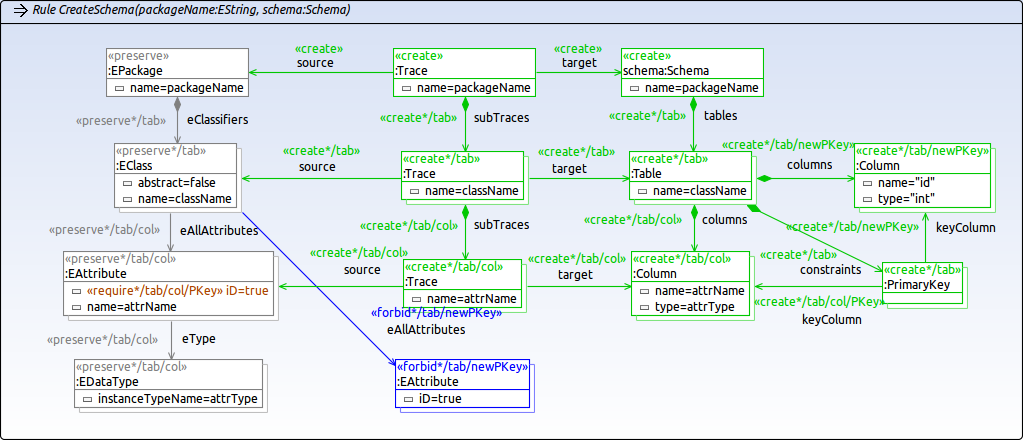
\includegraphics[scale=0.40,natwidth=1023,natheight=440]{Images/HenshinExample.png} 
	\caption{Henshin example}
	\label{figHenshinExample}
\end{figure}		

According to the developers of Henshin, the power of the underlying XML format exceeds the one of the graphical definitions and looks quite different when being compared to the visual representation. Therefore, a lot more complexity has to be expected when going deeper into this type of language.

After providing an overview of the \gls{ModelToModelTransformation} concepts found within the \glspl{DomainSpecificLanguage}, the language and tooling requirements are analyzed in the following paragraphs.

Considering the language requirements, some of them have been already fulfilled during the pre-selection. First of all, the selected languages are state of the art and have a detailed specification. The requirement of having independent \glspl{TransformationRule} and constructs is not fulfilled by operational textual \glspl{DomainSpecificLanguage} as they need an explicit \gls{TransformationRule} execution order to be defined. Finally, the ``simple start" is supported by all \gls{ModelToModelTransformation} \glspl{DomainSpecificLanguage}, because their design purpose was to provide a simple language for this domain. This excludes logical programming, since those languages are designed for more general purposes as already mentioned before.

On the other hand, the tooling requirements need to be inspected. As it is not the focus of this thesis to go deep into this matter, the explanations are short. The first requirement of providing a \gls{TransformationExecuter} was already fulfilled in the pre-selection. The second one of supporting non-user-interactive execution, i.e. providing a well documented and easy-to-use API for stand-alone execution, is  not fulfilled by any \gls{TransformationExecuter}. This is due to the fact that their primary purpose is to support a user in front of a modeling environment like Eclipse. Nevertheless, is was possible to create a ranking, in which the graph transformation engines marked the bottom line. The third requirement of providing high performance execution is not fulfilled by the \gls{AtlasTransformationLanguage} execution engine, since it is executed within its own, slow virtual machine. Providing a visual representation for \glspl{Trace} is provided by graph \glspl{TransformationExecuter}. Finally, an active community is more or less present for all of them. Especially well supported are \gls{AtlasTransformationLanguage} and the \gls{EpsilonTransformationLanguage}.

\textbf{Conclusion}: Overall, the declarative textual \glspl{DomainSpecificLanguage} in general and within this category the \gls{EpsilonTransformationLanguage} matched the requirements best compared to the others. The existing \gls{TransformationLanguage} and \glspl{TransformationExecuter} used in this thesis is the \gls{EpsilonTransformationLanguage}.

Besides selecting a \gls{TransformationLanguage} and \gls{TransformationExecuter} it is also necessary to create or select a language for the \glspl{MetaModel} themselves which is evaluated in the following sub-section.

% The most common modeling language in software engineering is the Unified Modeling Language (UML) \cite{umlInfra} and therefore it is recommendable to use it when possible.

\subsection{Meta-Model Language}\label{secModelLanguage}

To define patterns it is necessary to define the language of MM$_a$ and MM$_b$. For example, talking about a ``1:1 mapping between \glspl{Class}" assumes that there must be a \gls{Class} in both languages of MM$_a$ and MM$_b$ and also assumes that both share the same language. The refined problem domain overview in figure \ref{figProblemDomainOverviewRefined} contains this \gls{MetaMetaModel} MMM. It is on abstraction level M3 whereas the \gls{MetaModel} MM$_a$ and MM$_b$ are on level M2 and the concrete \glspl{Model} are on level M1.

\begin{figure}[htb]
	\centering
	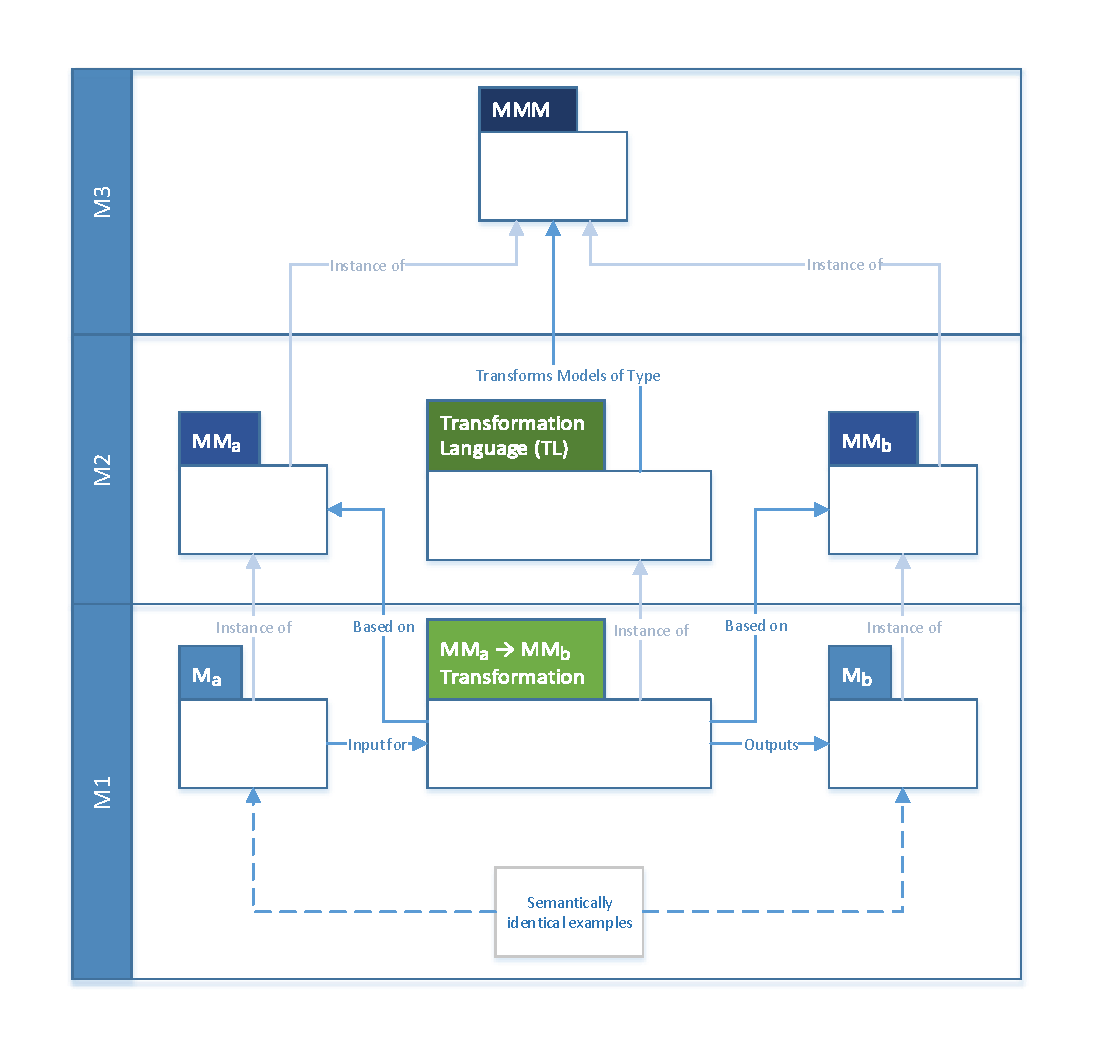
\includegraphics[scale=0.76, trim=0cm 1cm 0cm 1cm, clip=true]{Images/ProblemDomainOverviewRefined.pdf} 
	\caption{Problem domain overview refined - a ``MM$_a$ $\rightarrow$ MM$_b$ Transformation" has to be generated by using semantically identical input/output pairs. The input and output \glspl{MetaModel} MM$_a$ and MM$_b$, as well as the \gls{TransformationLanguage} conform to the meta-\gls{MetaModel} MMM.}
	\label{figProblemDomainOverviewRefined}
\end{figure}

An important distinction in the field of \glspl{ModelingLanguage} is the differentiation between the \gls{AbstractSyntax} and the \gls{ConcreteSyntax}. The \gls{AbstractSyntax} is a representation-independent language whereas the \gls{ConcreteSyntax} is a visually enhanced representation, optimized for the purpose of a specific language, with a mapping to the \gls{AbstractSyntax}. In this context, only the \gls{AbstractSyntax} is considered because it represents the generic foundation. 

As mentioned in section \ref{secRelatedWork}, the common language in \gls{SoftwareEngineering} is the \gls{UnifiedModelingLanguage} which is therefore used, among others, as a blueprint for the languages MM$_a$ and MM$_b$. In \gls{UnifiedModelingLanguage} the \gls{AbstractSyntax} can be described in the self-defining \glsfirst{MetaObjectFacility}. Hence, \gls{MetaObjectFacility} is the shared language MMM of MM$_a$ and MM$_b$ as it allows the use of \gls{UnifiedModelingLanguage} as well as other languages. 

Another method for defining languages on M2 is the light-weight extension mechanism of \gls{UnifiedModelingLanguage}, called profiles. The advantage of profiles is that everything what has been defined in \gls{UnifiedModelingLanguage} can be re-used. Since the support of profiles in the context of \glspl{ModelToModelTransformation} is not yet provided \cite{Randak2011}, this is not an option. As the thesis has the focus on automating \glspl{ModelToModelTransformation} the well supported \gls{MetaObjectFacility} is used.

As \gls{MetaObjectFacility} itself contains a large number of language constructs (\cite{ObjectManagementGroup2013}) which cover concepts that are not relevant for this thesis, it is reduced in such a way that it supports only the definition of basic structures. This is enough to specify basic languages on M2 and at the same time limits the complexity. It has to be pointed out that this is not a completely new language, but a reduced version of \gls{MetaObjectFacility} in order to avoid the undesired effects of self-defined languages described in the previous sub-section.

The illustration in Figure \ref{figMOFSimplified} shows the simplified \gls{MetaObjectFacility} definition in \gls{ConcreteSyntax} which allows the description of structures. Elements named ``\Glspl{Class}" are shown as boxes and their relations named ``\Gls{Association}" are shown as lines. 

\begin{figure}[!ht]
	\centering
	%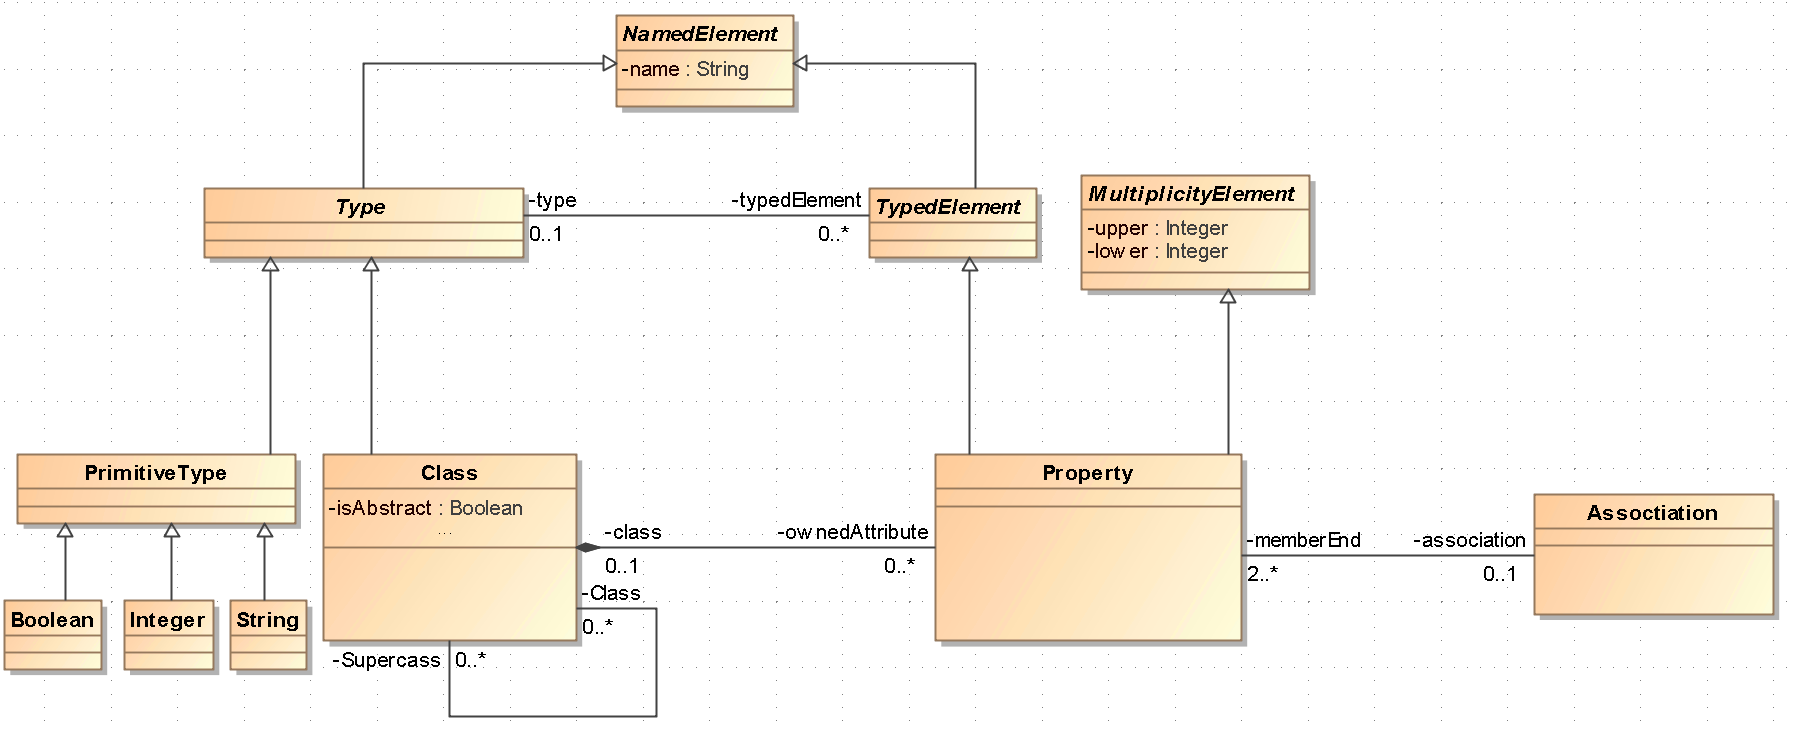
\includegraphics[scale=0.30,natwidth=1793,natheight=733]{Images/MOFSimplified.PNG} 
	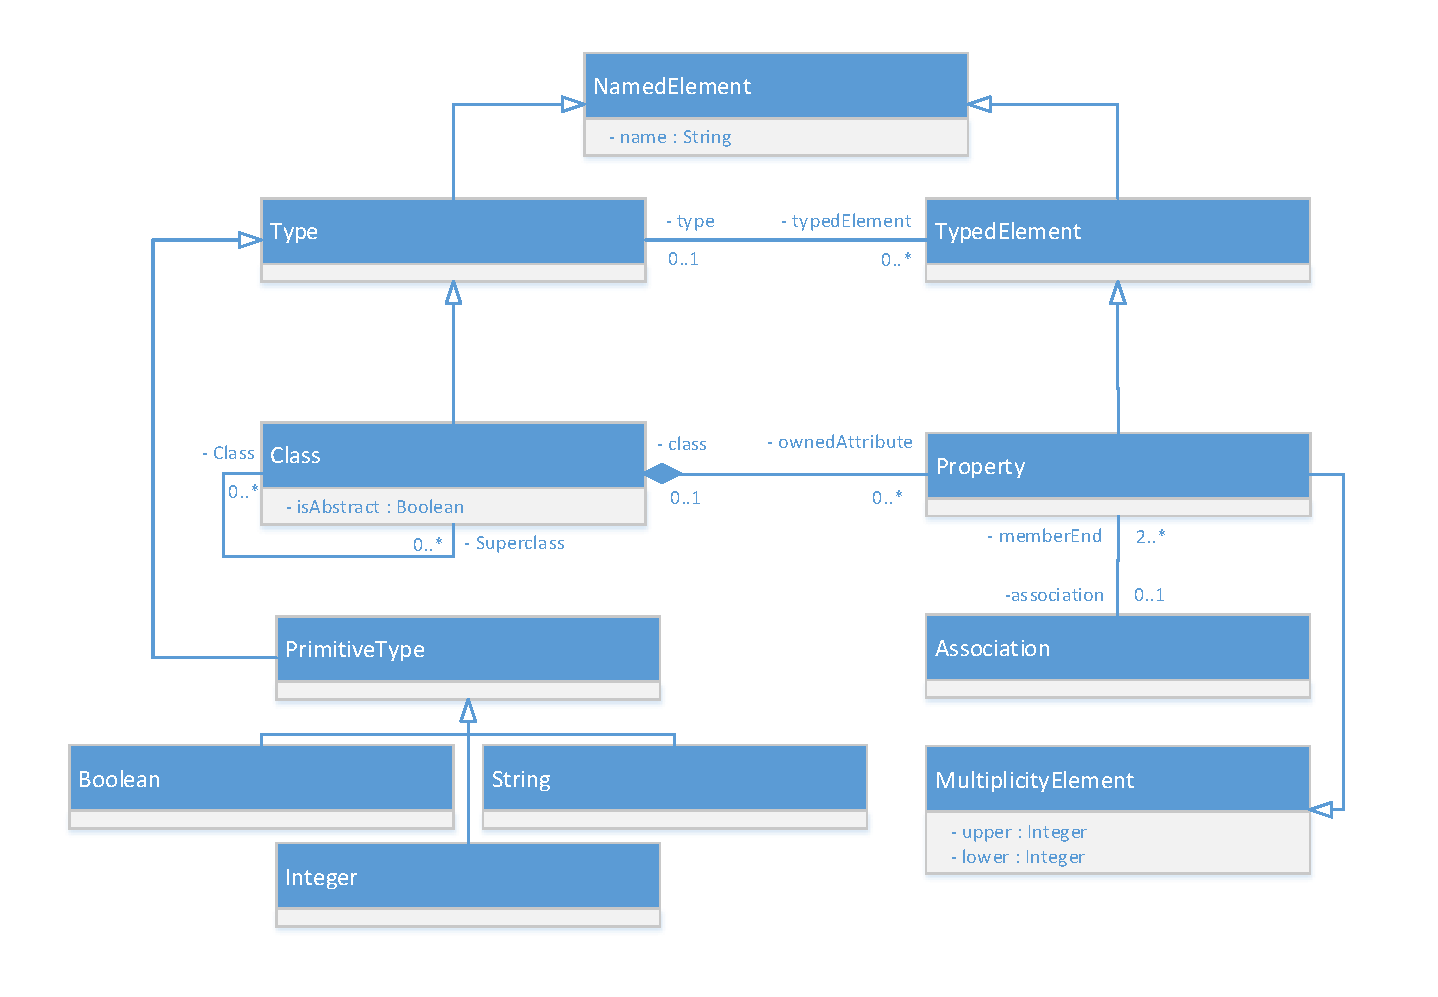
\includegraphics[scale=0.6, trim=0cm 1cm 0cm 1cm, clip=true]{Images/MOFSimplified.pdf} 
	\caption{\Gls{MetaObjectFacility} simplified}
	\label{figMOFSimplified}
\end{figure}

Additionally, ``\Glspl{Class}" consist of ``\Glspl{Property}" that may be the start or end of an ``\Gls{Association}" thereby being an ``MultiplicityElement" that describes how many of the associated ``\Glspl{Class}" are required and/or allowed i.e. ``0..1" is defined as ``lower=0" and ``upper=1" in the \gls{AbstractSyntax}. 

``\Glspl{Property}" may also be simple ``PrimitiveTypes" e.g. a ``String" or an ``Integer", or even ``\Glspl{Class}" which are visualized e.g. as ``upper: Integer" in the \gls{ConcreteSyntax} which is a \gls{Property} named ``upper" with a ``PrimitiveType". 

A \gls{Class} defines also a self-reference to describe the concept of inheritance by defining super-\glspl{Class} which derive everything to their sub-\glspl{Class}. In the \gls{ConcreteSyntax} this is visualized through lines with arrows at the end. 

``\Glspl{Class}" may also be marked as ``IsAbstract" which defines that they cannot be instantiated directly, only by deriving from it. In the simplified \gls{MetaObjectFacility} definition all ``\Glspl{Class}" with names in italic font are abstract. 

Finally almost everything must be able to get a proper name. Hence, most inherit from ``NamedElement".
%The Simplified \gls{MetaObjectFacility} definition is not completely self-describing as it uses role names for the ends of the association to improve the readability.

\gls{MetaObjectFacility} is sometimes not sufficient to describe a language, because it covers only the structural aspects without the possibility to specify i.e. constraints or calculated \glspl{Property}. Therefore, the \glsfirst{ObjectConstraintLanguage} \cite{ObjectManagementGroup2012} is defined in the \gls{UnifiedModelingLanguage}. It provides constructs to define conditions or calculated \glspl{Property}. Since those aspects would add more complexity and are not mandatory in basic languages, they are excluded to avoid unnecessary issues.

\subsection{Transformation Complexity}\label{secTransformationComplexity}

In the previous subsections an overview of \glspl{TransformationLanguage} has been presented as well as a definition of the M$_a$ and M$_b$ languages. The general approach of this thesis includes the construction of \glspl{MetaModel} for M$_a$ and M$_b$ which result in transformations ranging from simple to complex. Thus, this sub-section is focusing on the question how this construction can be performed systematically.

Up until now research does not provide such kind of systematic approach besides some indications (\cite{Strommer2007}, \cite{IvanGarcia-Magarino2009}, \cite{Patzina}). Nevertheless at least some basic categorizations regarding transformation complexity have been defined. But the perspective is usually based on the solution, the \gls{TransformationGenerator}, not the transformation.

Considering the analyzed related work (see section \ref{secRelatedWork}), an easy starting point are one-to-one \glspl{Object} transformations which do not require any pre-conditions and no \gls{Property} calculations. Both pre-conditions and \gls{Property} calculations may require complex queries, resulting in a more sophisticated \gls{TransformationGenerator}.

A further distinction was introduced by \cite{Strommer2007} between a so called ``Simple Mapping" and a ``Compound Mapping". Within the former one \gls{Class} of M$_a$ is mapped to exactly one of M$_b$. In the latter multiple \glspl{Class} of M$_a$ are mapped to multiple ones of M$_b$. Additionally, there are ``String Manipulations", which include all transformation operations, manipulating string-\glspl{Property} such as converting a character sequence to lower case before using it for a comparison. There were also some other categories which were not that generic, but rather specifically targeted at the approach. The mentioned definitions could also be found in other approaches and seem to be the unofficial standard regarding transformation complexity.

However, there are also other definitions which provide additional categories like \cite{IvanGarcia-Magarino2009} and \cite{Patzina}. The previously mentioned categories could be found here, too but also use e.g. the generation of constraints and the usage of negative examples as an input. Those categories are defined from a solution point of view. They do not directly describe what actually makes a transformation more or less complex and how to systematically evolve such a transformation.

Summarizing the existing research and merging it into the previously provided foundations is the next step. Foremost, the complexity of a transformation is related to the number and kind of relations between the \glspl{Class} on M2. For example, if a \gls{Class} of M$_a$ is always transformed into a specific \gls{Class} of M$_b$, this results in a simple 1:1 mapping. Assuming that the \gls{Class} of M$_a$ is transformed into two \glspl{Class} of M$_b$, this results in much more possible transformations, because the number of relations to be considered between \gls{Class} of M$_a$ and M$_b$ is 1:N and hence increases. Furthermore also N:1 and N:M are possible.

The same applies to the M1 level, where these kinds of relations are applicable. For example one \gls{Object} in M$_a$ can be transformed into two or more of the same type in M$_b$. This kind of transformation is usually not mentioned in the literature, but contains different challenges in the solution and should be handled separately. Considering the given example, there must be a definition especially for the number of the \glspl{Object} to be created. This can be either a value in an \gls{Object} in M$_a$ specifying the number of instances, a fixed number defined in the transformation or any kind of mathematical expression.

Besides the kind of relation, it has to be considered what could be related. Based on the definition of the simplified \gls{MetaObjectFacility} the possible relations, which can be defined in the mapping between M2 \glspl{Model}, are limited to the instances of non-abstract members of MMM in M3 which are \glspl{Class}, \glspl{Property}, \glspl{Association} and primitive types. Abstract members can be excluded because they are never directly used when creating a \gls{MetaModel} based on \gls{MetaObjectFacility} and are included in the non-abstract members via inheritance.

Basically, all of these can be related e.g. \glspl{Class} to \glspl{Class} with the defined relation possibilities like 1:N. Furthermore a transformation from a \gls{Class} to a \gls{Property} is possible, which increases the complexity. Finally a mixture can be necessary like transforming a \gls{Class} into a \gls{Property} and an \gls{Association}.


%=> define in scenarios!?
%
%c = \{c_1,c_2, ... c_n\}
%p = \{p_1,p_2, ... p_m\}
%a = \{a_1,_a2, ... a_o\}

%$$MM_\varsigma = \{ c \mid c -instanceOf-MOF Class \}$$
%$$MM_\rho = \{ p \mid p -instanceOf-MOF Property \}$$
%$$MM_\alpha = \{ a \mid a -instanceOf-MOF Association \}$$
%
%$$MM = \{c \mid c \in MM_\varsigma\} \cup \{p \mid p \in MM_\rho\} \cup \{a \mid a \in MM_\alpha\}$$
%$$MM_a,MM_b,MM_x \in MM$$
%
%$$M_\varsigma = \{ c \mid c -instanceOf-\varsigma, \varsigma \in MM_\varsigma \}$$
%$$M_\rho = \{ p \mid p -instanceOf-\rho, \rho \in MM_\rho \}$$
%$$M_\alpha = \{ a \mid a -instanceOf-\alpha, \alpha \in MM_\alpha \}$$
%
%$$M_x = \{c \mid c \in M_\varsigma\ \land c -instanceOf- MM_x\} \cup$$
%$$ \{p \mid p \in M_\rho\ \land p -instanceOf- MM_x\} \cup $$
%$$ \{a \mid a \in M_\alpha\ \land a -instanceOf- MM_x\}$$

%%%\
%%%
%%%\begin{enumerate}
%%%	\item One-to-One on M2 and M3 = $\{(a_A,b_B) \mid A \in {MM}_a, B \in {MM}_b\, a \in {M}_a, b \in {M}_b$
%%%	\item One-to-One on M2 and M3 - context sensitive = \\$\{(A,B,c) \mid A \in {MM}_a, B \in {MM}_b, c \in Constraints\}$
%%%	\item One-to-Many on M3 = $\{(A,B_1,..,B_n) \mid A \in {MM}_a, B \in {MM}_b \}$
%%%\end{enumerate}
%p -> p
%a -> a
%
%c -> p
%c -> a
%p -> c
%p -> a
%a -> c
%a -> p
%
%\\


%c|a(x) -> ...
%c|b(x) -> ...
%
%
%
%1:N - M3
%c -> c_1, c_2, c_n
%...
%
%1:N - M2
%c -> c, p
%c -> c, p, a
%...
%
%1:N - M2 + M3
%c -> c_1, c_2, p_1
%...
%
%1:N - M2 and/or M3 - context sensitive
%c|a(x) -> ...
%c|b(x) -> ...
%
%
%
%
%N:1 - M3
%...
%
%N:1 - M2
%...
%
%N:1 - M3 + M2
%...
%
%N:M - M3
%...
%
%N:M - M2
%...
%
%N:M - M2 + M3
%...
%
%...



%%%$$ \{(c_1,p_1,a_1),...,(c_n,p_m,a_o)\} X \{c,p,a\}

This idea might help to systemically develop \glspl{MetaModel} for M$_a$ and M$_b$ which result in transformations with different complexity levels. Though, it remains incomplete as in general a transformation can be more difficult e.g. when considering the computation of \glspl{Property} or pre-conditions for the application of a mapping.

\section{Meta-Heuristic Optimization Algorithms}\label{secAlgorithms}

In contrast to the most existing approaches, this thesis is trying to solve the generation of \glspl{ModelToModelTransformation} without using a direct deduction from manually provided links or recorded user transformations. Instead, the idea is to utilize meta-heuristic optimization algorithms to construct the transformation. As an input, only the manually created \glspl{Model} M$_a$ and M$_b$ are used. They are the reference for correctness of the created solution. Therefore, algorithms are required that are able to cover large \glspl{SearchSpace} because a \gls{ModelToModelTransformation} can become complex with these assumptions (see sections \ref{secRelatedWork} and \ref{secTransformationComplexity}).

The meta-heuristic optimization algorithms, that are analyzed for possible applications, are from the field of \glspl{SwarmIntelligentAlgorithm} and \glspl{EvolutionaryAlgorithm}.

The fundamental requirement to apply such algorithms is the reduction of the given problem. Every algorithm expects a certain \gls{Encoding} of the problem, with different restrictions, which is used to represent a \gls{CandidateSolution} and thereby defines the \gls{SearchSpace} (\cite{holland75},\cite{Dorigo},\cite{Cook1997}).

In general the algorithms are categorized into combinatorial and generative (\cite{holland75},\cite{Dorigo},\cite{Cook1997}). The former requires that the \gls{Encoding} of the problem consists of a finite set of building blocks that can be assembled to a solution. The algorithm either uses a discrete approach, to pick any blocks or a continuous one, i.e. weights or probabilities are assigned to the blocks. The latter category is used to create something from scratch without the need to have a finite set of building blocks.

Without having any guidance in a \gls{SearchSpace} each algorithm would perform a random search. Hence, the general concept is to provide a so-called \gls{FitnessFunction} to rate \glspl{CandidateSolution}. Having this rating as a foundation, \glspl{Operator} are required to modify the \glspl{CandidateSolution} to make steps through the \gls{SearchSpace} (\cite{holland75},\cite{Ashlock2004}). Those terms are not used that frequently in the field of \glspl{SwarmIntelligentAlgorithm} than in \glspl{EvolutionaryAlgorithm}, but the general concepts also apply there.

The steps in the \gls{SearchSpace} can be separated into \gls{LocalSearch} and \gls{DistantSearch} (\cite{Ashlock2004}). The former search behavior is moving from \gls{CandidateSolution} to \gls{CandidateSolution} within the neighborhood and thereby making small, local steps. Whereas the \gls{DistantSearch} is performing large steps, hence moving faster to completely different \glspl{CandidateSolution}. This behavior is usually more unpredictable and irregular and therefore more challenging. 
In order to identify the optimal solution a combination of both can be beneficial in terms of performance or can be even necessary to avoid getting trapped in a \gls{LocalOptimum} (\cite{Kessentini2010},\cite{holland75}). \Gls{DistantSearch} may be exploring the \gls{SearchSpace} and when an area in the search space seems promising then \gls{LocalSearch} is used to exploit it and find the optimal solution (\cite{Kessentini2010}).

In this thesis, the algorithms considered for possible applications are \glspl{SwarmIntelligentAlgorithm} and \glspl{EvolutionaryAlgorithm}. Both are presented in the following subsections in a survey-like manner.

\subsection{Swarm-Intelligent Algorithms}\label{secSwarmIntelligentAlgorithms}

\textbf{\Gls{AntColonyOptimization}} \cite{Dorigo} is inspired by the behavior of \glspl{Ant} when looking for \glspl{FoodSource}. Initially it has been used to solve the Traveling Salesman Problem (TSP), but is also applicable to scheduling or assignment problems or similar graph based problems. The idea is to mimic the behavior of \glspl{Ant}, which are creating a \gls{PheromoneTrail} while exploring the \gls{SearchSpace}. In the case many \glspl{Ant} use the same path, the \gls{PheromoneTrail} is intensified and becomes more attractive to other \glspl{Ant}. But such a trail evaporates over time, hence a longer path is less likely be preferred as it takes a longer time to travel to the \gls{FoodSource} and back compared to a shorter path, where the trail does not evaporate to the same extend. Therefore, frequently used paths are enforced and preferred by other \glspl{Ant}, resulting finally in the shortest path to the \gls{FoodSource}.

This algorithm might be applicable when using a combinatorial approach, i.e. a food source is a complete transformation and the way to the \gls{FoodSource} defines the decisions made. This might result not only in a working solution but also in the smallest solution with a minimal number of constructs.

\textbf{\Glsfirst{ParticleSwarmOptimization}} \cite{Kennedy1995} mimics the behavior of bird flocks or fish schools. Basically a \gls{CandidateSolution} is a \gls{Particle} in an n-dimensional \gls{SearchSpace}. Each \gls{Particle} has a velocity and direction hence moving around. After each time-step every \gls{Particle} evaluates its own position with the \gls{FitnessFunction} and updates his own best-known position and also the globally best-known one. Afterwards, the direction and velocity of each \gls{Particle} are updated based on the new information.

As the \gls{Encoding} is a n-dimensional vector the algorithm is applicable in a combinatorial approach. The first idea would be to divide a \gls{ModelToModelTransformation} into partial transformations representing a dimension.

%\textbf{BEECLUST algorithm} \cite{Bodi2009} TODO interesting? reduced number of fitness function evaluations?

\subsection{Evolutionary Algorithms}\label{secEvolutionaryAlgorithms}

\Glspl{EvolutionaryAlgorithm} are using so-called \glspl{Genotype} as a language for the \gls{Encoding} of the given problem which consists of \glspl{Gene} (\cite{holland75},\cite{Ashlock2004}). The actual \gls{CandidateSolution} is the \gls{Phenotype} representing the observable behavior. Both together are forming an \gls{Individual}, which is part of a \gls{Population}. In the context of \glspl{ModelToModelTransformation} such a \gls{Phenotype} is most likely a transformation. \Glspl{GeneticOperator} are modification strategies for the \glspl{Genotype} which add the actual evolutionary aspect by changing \glspl{Genotype} in a certain way and thereby creating new \glspl{CandidateSolution}. 

\begin{figure}[htb]
	\centering
	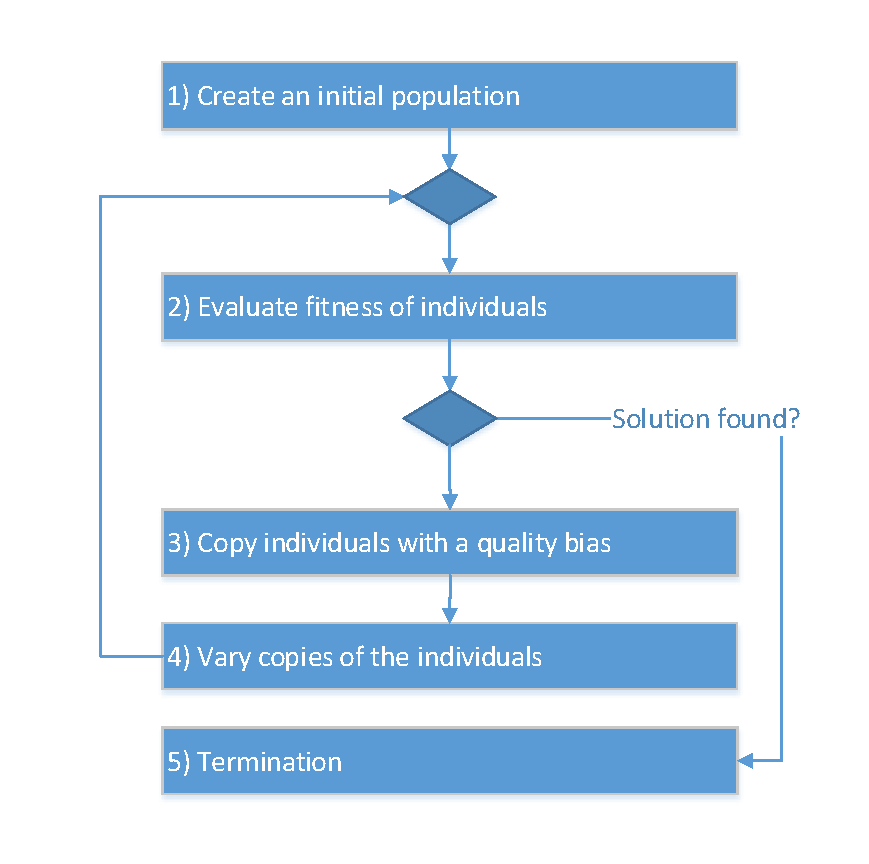
\includegraphics[scale=0.6, trim=0cm 1cm 0cm 1cm, clip=true]{Images/AlgorithmEA_GeneralOverview.pdf} 
	\caption{Evolutionary algorithm - general overview (\cite{Ashlock2004})}
	\label{figEvolutionaryAlgorithmGeneralOverview}
\end{figure}

Figure \ref{figEvolutionaryAlgorithmGeneralOverview} shows the basic control flow of an \gls{EvolutionaryAlgorithm} derived from \cite{Ashlock2004}. The first step is to create an initial \gls{Population} with a defined size representing the first \gls{Generation}. The \glspl{Individual} can be either the result of a random generation or the result from another algorithm.
The evolutionary loop then starts with the evaluation of the \glspl{Individual} using the \gls{FitnessFunction}. In the case a solution is found, the loop ends. Afterwards solution candidates are picked using a \gls{SelectionStrategy}, then are copied thereby eliminating others chosen by a \gls{ReplacementStrategy} in order to maintain a fixed \gls{Population} size. Both strategies are based on the fitness.
The final step of the loop variates the \gls{Population} by applying \glspl{GeneticOperator} on the copied \glspl{Individual}.

After describing the general behavior, a rough overview of the crucial aspects is provided in the following paragraphs.

First, the basic \glspl{SelectionStrategy} are introduced. Within \gls{RouletteWheelSelection} the probability for an \gls{Individual} to be chosen, is the proportion of its fitness to the sum of all fitness values. \Gls{TournamentSelection} creates subsets of the whole \gls{Population} and choses the best one. The size of the subset defines the selection pressure, i.e. a large subset reduces the chance for \glspl{Individual} with bad fitness to be chosen. A high selection pressure reduces the \gls{GeneticDiversity} as \glspl{CandidateSolution} with bad fitness are less likely to be exploited further.

\Glspl{ReplacementStrategy}, or also called child insertion methods, maybe of different kinds as well. A common strategy is \gls{Elitism}, where a certain number of best \glspl{Individual} is kept. Thereby, it ensures that the overall fitness never decreases but increases the chance of getting trapped in a \gls{LocalOptimum}. Those strategies may also be directly related to the \glspl{SelectionStrategy}, i.e. within the subset of a \gls{TournamentSelection} the \gls{Individual} having the worst fitness is replaced by an offspring of the one with the best fitness.

Two schemata exist for \glspl{GeneticOperator}. The first one is an unary \gls{Mutation} operator that creates a variation of an existing \gls{CandidateSolution}. It changes each \gls{Gene} of a selected \gls{Individual} with a certain probability. Basically, the idea is to perform a \gls{LocalSearch} which requires \gls{StrongCausality}. A mutation is a small change in the \gls{Genotype} and should only result in a small change in the \gls{Phenotype}. The second operator is the binary \gls{Crossover} which is applied to pairs of selected \glspl{Individual} and re-combines them to a new one. Hence, the new \gls{Individual} is located between its parents in the \gls{SearchSpace} which might be a large step. Therefore, this is a \gls{DistantSearch}.

\Glspl{EvolutionaryAlgorithm} can be quite different depending on the concrete approach. The most important and relevant ones for this thesis are presented to provide an overview for the algorithm design.

\textbf{\Gls{EvolutionaryStrategy}} \cite{rechenberg73} uses only \gls{Mutation} as an \gls{GeneticOperator}. The \glspl{Genotype} is typically based on floating-point arrays. When mutating the array, usually a normally distributed random value is added. An application of this concept might be possible in a combinatorial approach. It is probably difficult because creating a transformation based on floating point numbers has to overcome a large semantical gap.

In the case a \gls{ModelToModelTransformation} can be divided into several independent parts and each part is assigned a weight, this might be applicable.

\textbf{\Gls{GeneticAlgorithm}} \cite{holland75} is using \gls{Mutation} and \gls{Crossover} based on discrete \glspl{Genotype} (e.g. binary strings). Thus, a \gls{Mutation} is usually a bit-flip and a recombination is a one-point or two-point \gls{Crossover}.
The basic one-point \gls{Crossover} splits the parent \glspl{Genotype} into two parts at the same ``point". The new \gls{Genotype} then uses the left hand side of the first parent and the right hand side of the second parent. An extension is the two-point \gls{Crossover} which splits the parents into three parts at two ``points". Therefore, the new \gls{Genotype} is based on three parts where two are from the same parent.

This algorithm might also be applicable in a combinatorial approach.

\textbf{\Gls{GeneticProgramming}} \cite{koza92} is based on tree-representation of programs as the \gls{Genotype} which is usually the \gls{AbstractSyntaxTree}. The \gls{Mutation} and \gls{Crossover} \glspl{GeneticOperator} are therefore changing the \gls{AbstractSyntaxTree}.

Since the \gls{ModelToModelTransformation} is a program, this algorithm is presumably applicable. The major challenge is probably the \gls{LocalSearch}, as a small change in the \gls{AbstractSyntaxTree} might create a major semantic change in the program resulting in a major change in the \gls{FitnessFunction}.

\subsection{Application to Model Transformation By Example}\label{secApplicationToMTBE}

The previous subsections indicated for each algorithm a rough idea how an application to \gls{ModelTransformationByExample} could be achieved. Overall most of the presented algorithms are targeted at combinatorial problems. In order to apply those, the incomplete described problem of \gls{ModelToModelTransformation} has to be mapped to a complete problem with precise dimensions. Thereby, this reduction introduces limitations which will render the algorithm most likely in-adaptable for scenarios that are not part of this thesis. On the contrary, a \gls{GeneticProgramming} is the only one that is targeted at creating tree-based representations of programs. Hence, instances of a \gls{TransformationLanguage} can be created by such an algorithm without a reduction. However, the complexity of the presented \gls{TransformationLanguage} is an issue, that does not create difficult requirements for the \gls{Encoding} within a \gls{GeneticProgramming}, but for the \glspl{GeneticOperator} and the \gls{FitnessFunction}.

\chapter{Solution Approach}\label{chapAlgorithmicApproach}

After presenting the foundations of \gls{ModelTransformationByExample}, \glspl{ModelToModelTransformation} and meta-heuristic optimization algorithms, this chapter explains the solution approach. At first, the requirements are refined in section \ref{secRequirements}. Afterwards, the decision for the meta-heuristic optimization algorithm type is explained in section \ref{secAlgorithmTypeSelection}. Finally, an overview of the solution is presented in section \ref{secSolutionOverview} followed by a description of the used design and development process in section \ref{secDesignAndDevelopmentProcess}.

\section{Requirements}
\label{secRequirements}

The refined requirements are presented in this section based on the results of the previous chapter. At first a summary of the most important findings is listed:

\begin{itemize}
	\item The chosen definition of \gls{ModelTransformationByExample} provides little information as a guidance for the algorithm (see subsection \ref{secRelatedWorkConclusions}).
	\item A generic and precise definition of \gls{ModelToModelTransformation} is not provided by any \gls{TransformationLanguage} (see subsection \ref{secExistingModelTransformationLanguagesAndTools}). Such a definition can also not be derived from the \gls{MetaMetaModel} language \gls{MetaObjectFacility} within this thesis (see subsection \ref{secTransformationComplexity}).
\end{itemize}

The first finding results in a large and intangible \gls{SearchSpace}. Whereas, the second finding renders a complete solution of the chosen \gls{ModelTransformationByExample} problem impossible within this thesis. The refined requirements are shown in figure \ref{figRequirements} and listed in the following:

\begin{figure}[ht!]
	\centering
	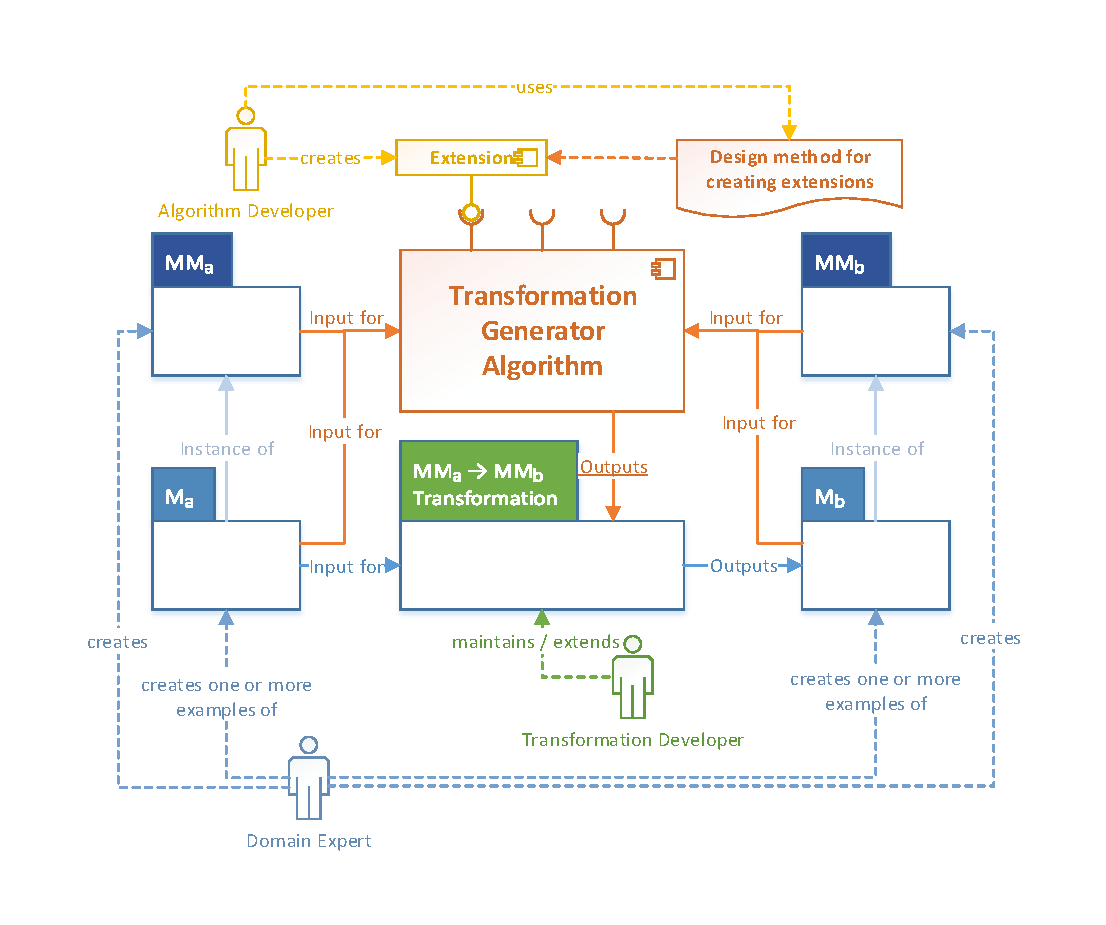
\includegraphics[scale=0.8, trim=0.5cm 1cm 0.5cm 1cm, clip=true]{Images/Requirements.pdf}
	\caption{Requirements - An extensible algorithm must be defined including a design method for creating extensions}
	\label{figRequirements}
\end{figure}

\begin{itemize}
	\item The algorithm creates a ``MM$_a$ $\rightarrow$ MM$_b$ Transformation" based on given \glspl{MetaModel} MM$_a$ and MM$_b$ provided by a domain expert. 
	\item It is guided by manually created M$_a$ - M$_b$ example-pairs, also created by a domain expert. No further information is provided like details about the mapping from M$_a$ to M$_b$.
	\item Since a complete algorithm cannot be created due to the incomplete definition of \glspl{ModelToModelTransformation}, the algorithm cannot guarantee a solution. Hence, the algorithm must be extensible by providing generic extension parameters.
	\item The algorithm must consider large \glspl{SearchSpace}.
	\item A design method for creating extensions must be defined. It guides the algorithm developer. In particular, the method must consider the problem of non-termination in large \glspl{SearchSpace}.
	\item The created ``MM$_a$ $\rightarrow$ MM$_b$ Transformation" might not be a complete solution, since the algorithm is incomplete. Thus, the transformation must be maintainable by a transformation developer.
	\item A solution for the transformation scenarios defined in chapter \ref{chapM2MScenarios} must be found within a few hours, which is considered an acceptable time.
\end{itemize}

\section{Meta-Heuristic Optimization Algorithm Type Selection}
\label{secAlgorithmTypeSelection}

Before presenting the solution overview, this section at first explains the decision for an algorithm type. This decision has an impact on all other aspects of the algorithm design. As a result of the previous insights there are two possible directions which are presented in the following.

The first one (Direction A) is to use the definition of a \gls{TransformationLanguage} to create instances of itself. The second one (Direction B) is to divide the general problem of \glspl{ModelToModelTransformation} into smaller units, which are then being solved by meta-heuristic optimization algorithms.

While direction A is the more direct one, because it could more or less immediately be tackled by a \gls{GeneticProgramming} (see subsection \ref{secEvolutionaryAlgorithms}), it has also the greater chance of facing the problem of non-termination very soon. This is due to the fact that \glspl{TransformationLanguage} are complex, which has been outlined in subsection \ref{secExistingModelTransformationLanguagesAndTools}. Combined with the results of section \ref{secAlgorithms} the definition of a \gls{FitnessFunction}, which converges to a solution might become difficult. Most of the created instances are probably far away from any kind of solution ending up in a random search.

This issue could be avoided in the fist place by direction B. The idea is to split the problem of \glspl{ModelToModelTransformation} into different, algorithmic-friendly sub-problems or units. For example one unit might be matching \glspl{Class} from M$_a$ to M$_b$ and another one matching the \glspl{Property}. The former may be a combinatorial problem while the latter is a generative one. So an assignment of the ideal algorithm for each unit is possible.

Nevertheless, also direction B has two major downsides. On the one hand, the overall aggregation of the units is an ``ordinary" algorithm that has to be created from scratch. This algorithm is not based on a meta-heuristic and hence, lacks a theoretical foundation. On the other hand, creating units is a huge challenge on its own. In particular, there is a risk that the algorithm-friendly language has fundamental limitations, which renders it useless in common scenarios that have not been considered in the design phase. Consequently, an extension might require changing the existing algorithm. Thus, the extensibility of the algorithm with an acceptable effort cannot be guaranteed. Furthermore, following this approach leads to a focus on the definition of a \gls{TransformationLanguage} and the aggregation of the units and not on the actual algorithms.

After looking at the advantages and disadvantages of both directions the risk of designing an own algorithm-friendly, unit-based \gls{TransformationLanguage} has been considered as too high, because it might very likely exceed the scope of this thesis and move the focus in a different direction. Hence, the decision is to take direction A using a \gls{GeneticProgramming}. 

% with the restriction, to avoid the non-termination issue as far as possible. Only \glspl{Class}, \glspl{Association} and \glspl{Property} without any calculations are transformed. The calculation of the latter introduces, as already mentioned in section \ref{secRelatedWork}, at lot of additional complexity. In order to link \glspl{Class} of MM$_a$ to MM$_b$ it is assumed that there is a \gls{Property} ``Name" that is equal in \glspl{Object} of M$_a$ and M$_b$ for semantically identically \glspl{Class} (see section \ref{secRelatedWork}).

%If the algorithm works, then \glspl{Property} are taken into account. Otherwise, it is the task of the developer to extend the transformation. An additional requirement in direction A is therefore that the result must be readable and maintainable manually because it might be incomplete. This is considered when designing and evaluating the algorithm.

\section{Solution Overview}
\label{secSolutionOverview}

This section provides an overview of the solution. At first the general concept is explained and afterwards an overview of the central entities of the solution. As explained within the requirements, the algorithm will be incomplete, but must be extensible as well as the created \glspl{ModelToModelTransformation}. Furthermore, the large \gls{SearchSpace} must be considered since it might prevent the algorithm from terminating with a solution at all or in an acceptable time.

\begin{figure}[ht!]
	\centering
	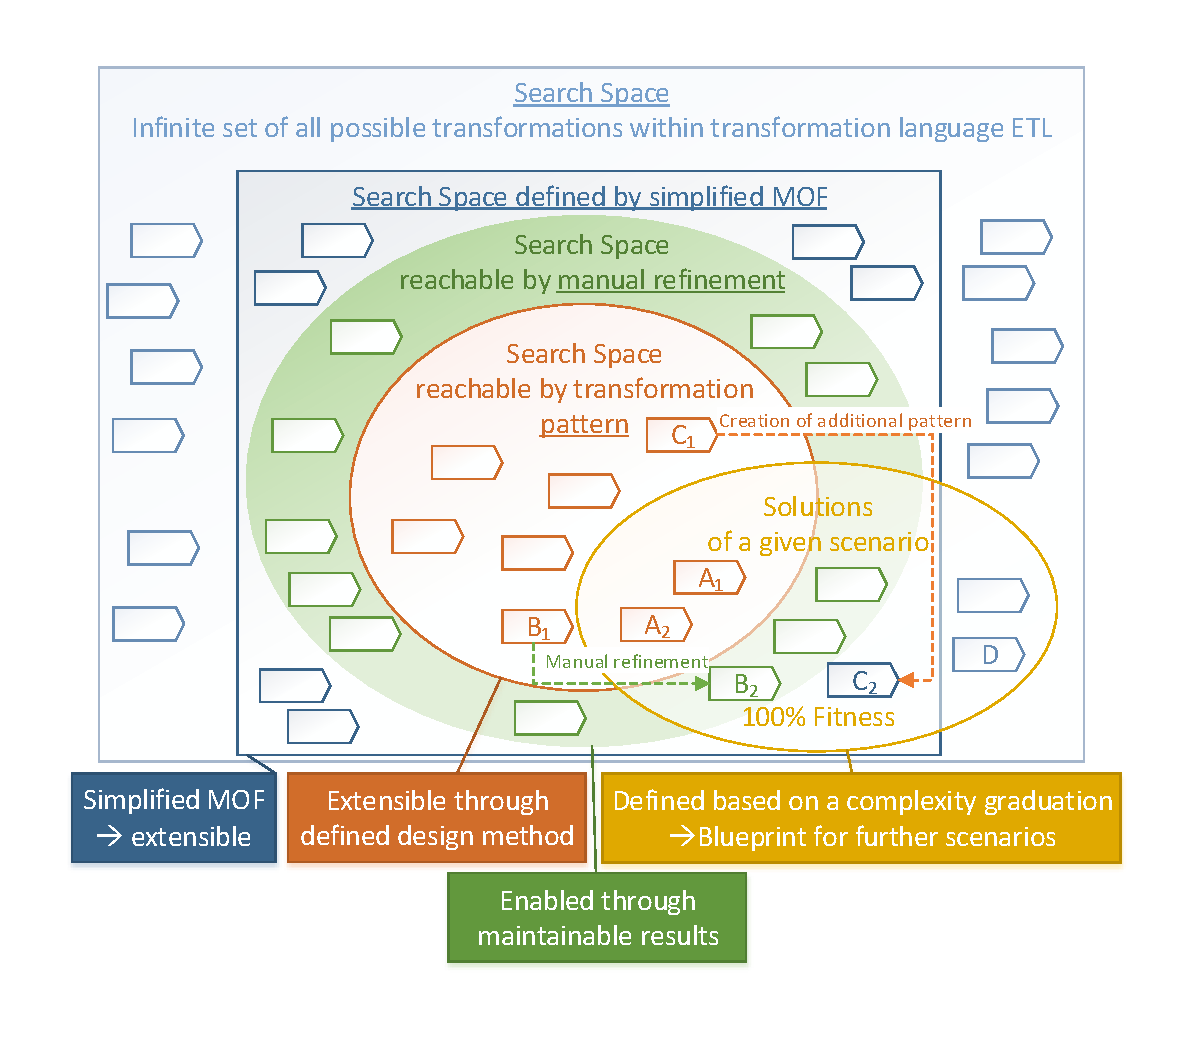
\includegraphics[scale=0.7, trim=0cm 1cm 0cm 1cm, clip=true]{Images/SearchSpaceDivideAndConquer.pdf} 
	\caption{Search Space - Overview of the divide-and-conquer approach}
	\label{figSearchSpaceDivideAndConquer}
\end{figure}

Figure \ref{figSearchSpaceDivideAndConquer} provides an overview of the general concept to fulfill those requirements. The presented key ideas are listed in the following: %It shows transformations as small blocks. Solutions for a given transformation scenario can be

\begin{itemize}
\item The whole \gls{SearchSpace} is defined by the infinite set of all possible transformations within the \gls{EpsilonTransformationLanguage}.
\item In order to limit the possible transformations considered in this thesis, the \gls{MetaMetaModel} language \gls{MetaObjectFacility} is simplified (see subsection \ref{secModelLanguage}). Thereby, the possible \glspl{MetaModel} are limited which can be solved by a limited number of transformations. The simplified \gls{MetaObjectFacility} is the foundation for the systematic construction of the representative transformation scenarios. Within figure \ref{figSearchSpaceDivideAndConquer}, the solution D of the given transformation scenario is therefore out-of-scope. Nevertheless, the simplified \gls{MetaObjectFacility} can be extended towards \gls{MetaObjectFacility}.
\item The \gls{GeneticProgramming} is based on transformation patterns, which are the foundation of its \glspl{GeneticOperator}. Those patterns are a small subset of the \gls{EpsilonTransformationLanguage}. Therefore, they cannot create all solutions for a given scenario. In figure \ref{figSearchSpaceDivideAndConquer} only the solutions A$_1$ and A$_2$ can be created by the algorithm. 
\item Transformation patterns are well-defined transformation concepts and avoid creating incomprehensible solutions. Thereby, a transformation developer can for example modify the transformation B$_1$ into B$_2$. The former was close to the solution, while the latter is a 100\% solution of the given scenario. In general, a manual modification could result in any transformation i.e. also C$_2$. This requires more knowledge and effort compared to small modifications which are therefore only expected.
\item Transformation patterns can be extended using the defined design method. For example, the algorithm might terminate with the transformation C$_1$ which is not a solution of the given scenario. By adding an additional pattern, the algorithm becomes capable of modifying this transformation to C$_2$, which is a solution. 
\item Furthermore, most of the transformations in the \gls{SearchSpace} are likely to produce low-quality output. It can not be distinguished with the given inputs for the algorithm. Hence, the algorithm has no guidance and the termination with a solution - even when theoretically reachable - is unlikely. The patterns also limit this problem, when designed according to the specified design method.
\end{itemize}

\begin{figure}[ht!]
	\centering
	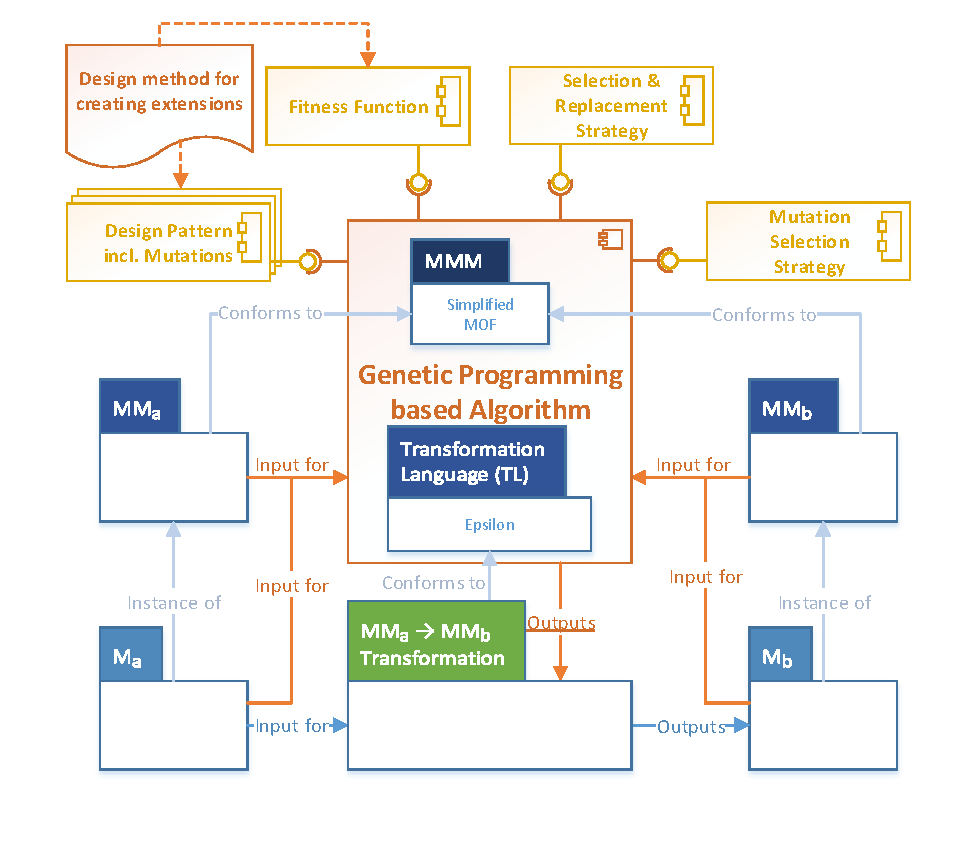
\includegraphics[scale=0.8, trim=0.5cm 1.2cm 0.5cm 0cm, clip=true]{Images/Solution.pdf}
	\caption{Overview of the central entities of the solution}
	\label{figSolution}
\end{figure}

After explaining the general concept, the central entities of the solution are presented in figure \ref{figSolution}. The algorithm is based on a \gls{GeneticProgramming} as decided in the previous section \ref{secAlgorithmTypeSelection}. The input and output \glspl{MetaModel} are instances of the simplified \gls{MetaMetaModel} \gls{MetaObjectFacility} (see subsection \ref{secModelLanguage}). Created ``MM$_a$ $\rightarrow$ MM$_b$ Transformation" conform to the selected \gls{TransformationLanguage} \gls{EpsilonTransformationLanguage} (see subsection \ref{secExistingModelTransformationLanguagesAndTools}). Besides the previously mentioned transformation patterns also other aspects of the algorithm are exchangeable and/or extensible components. Transformation patterns are the foundation for the \glspl{Mutation} required by the \gls{GeneticProgramming}. Since there are many patterns resulting in many \glspl{Mutation}, a mutation selection strategy is required. The \gls{FitnessFunction} is necessary to rate transformations created by the algorithm. As explained in subsection \ref{secEvolutionaryAlgorithms}, the algorithm is based on a \gls{SelectionStrategy} and \gls{ReplacementStrategy}, which is also an exchangeable component.

The design method describes the creation of additional transformation patterns and the required extensions of the \gls{FitnessFunction}. Since additional patterns extend the reachable transformations, those transformations also create other types of output \glspl{Model}. Hence, the \gls{FitnessFunction} which rates the transformation depending on the output, must be adopted to reflect the new types as well.

\section{Design and Development Process}
\label{secDesignAndDevelopmentProcess}

Since this thesis tries to solve a software engineering problem with a meta-heuristic optimization algorithm using a new approach, there is no reference design process available, yet. Therefore, this section provides an overview of the followed design and development process shown in figure \ref{figDevelopmentProcess}. The x-axies of the matrix contains the software development process phases Design, Implementation, Unit Test and Integration Test / Evaluation. On the y-axis are the entities of the algorithm. The size of each step from one to nine in figure \ref{figDevelopmentProcess} indicates the spent effort. The following list provides an overview of the design and development process of the algorithm entities:

\begin{figure}[htb]
	\centering
	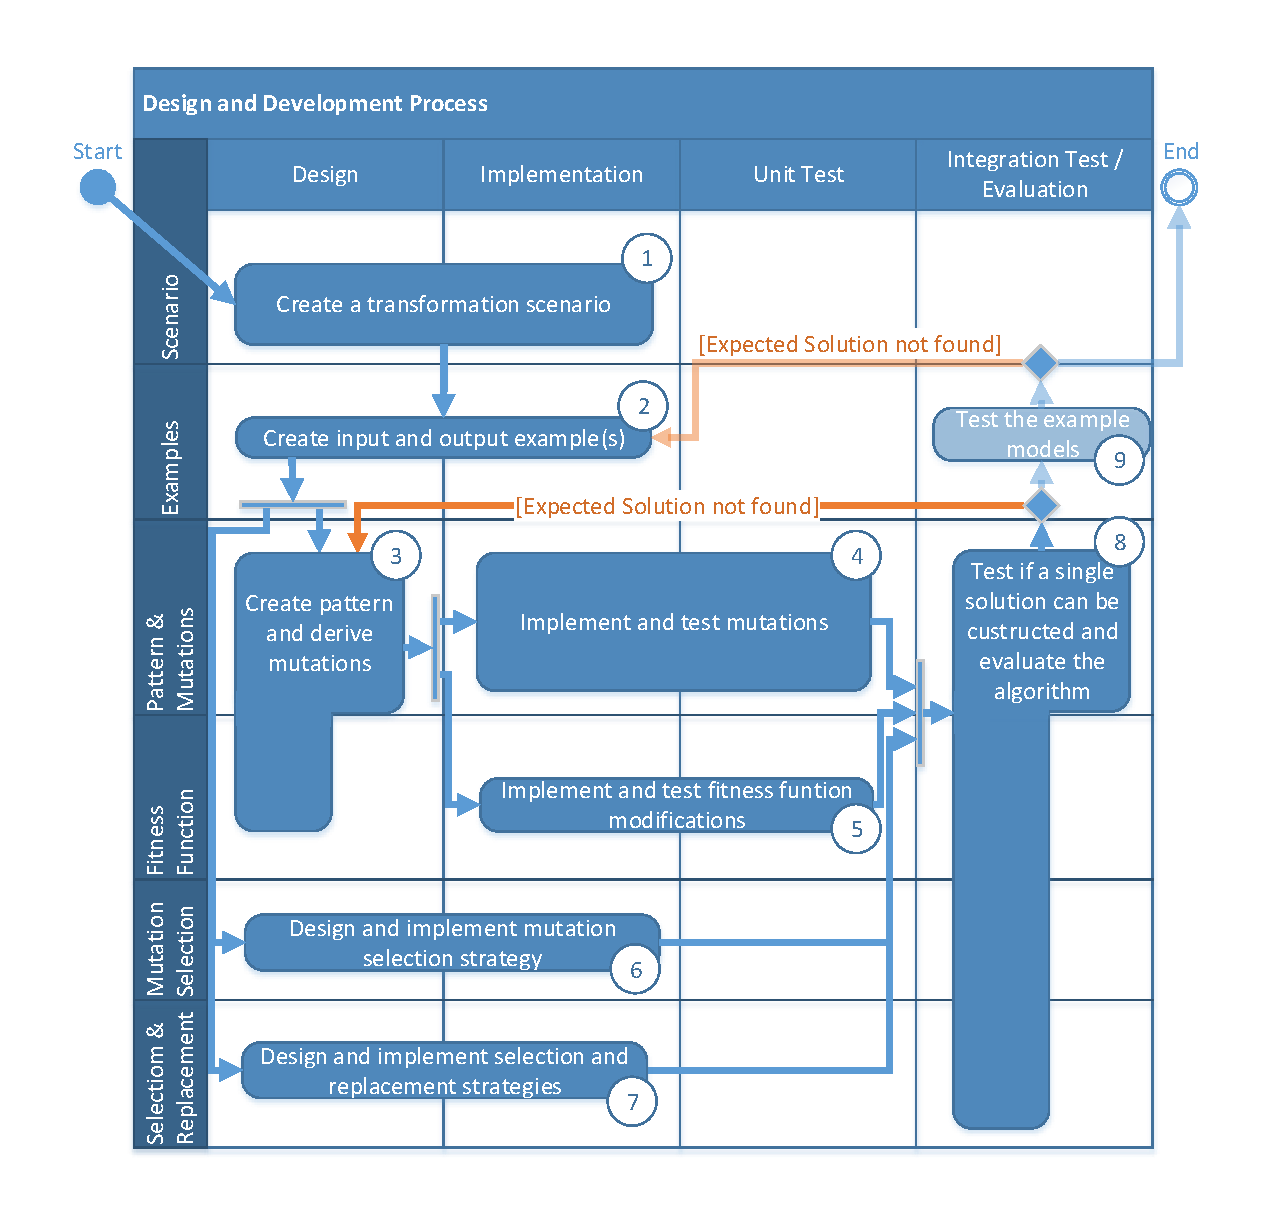
\includegraphics[scale=0.7, trim=0cm 1cm 0cm 1cm, clip=true]{Images/DevelopmentProcess.pdf} 
	\caption{Design and development process - overview of the created entities and phases. The size of the activities indicates the effort.}
	\label{figDevelopmentProcess}
\end{figure}

\begin{enumerate}
	\item Create a transformation scenario. It includes the transformation problem defined by two \glspl{MetaModel}. Furthermore, a reference transformation from the first to the second \gls{MetaModel} is specified as a guideline for the pattern design. In order to control the complexity of the scenario, the complexity analysis presented in subsection \ref{secTransformationComplexity} is used. The created scenarios are explained in chapter \ref{chapM2MScenarios}.
	\item For each scenario, at least one input and expected output \gls{Model} has to be created. Those are also presented in chapter \ref{chapM2MScenarios}.
	\item Afterwards, the reference transformation is analyzed and missing transformation patterns are added or existing patterns are extended. Based on the patterns, the \glspl{Mutation} are derived which are used by the algorithm. Also the \gls{FitnessFunction} is extended to reflect the new kinds of output created by the added \glspl{Mutation}. The design method required to create these entities is presented in section \ref{secMutationAndFitnessFunctionDesignProcess}, the implemented patterns are described in \ref{secPatternAndMutations} and the \gls{FitnessFunction} in section \ref{secFitnessFunctions}.
	\item Following the software development process, the \glspl{Mutation} are implemented and tested individually (see section \ref{secRealizationOfMutations} and section \ref{secMutationProcess}).
	\item The same applies to the \gls{FitnessFunction}, which is also tested using selected transformations derived from the reference transformation (see section \ref{secMutationProcess}).
	\item The Mutation Selection Strategies have a design and implementation phase, but are not tested individually. They are relatively simple and the effect is only observable in the integration test of all components (see section \ref{secMutationSelectionStrategies}).
	\item The same applies to the Selection and Replacement Strategies (see section \ref{secSelectionReplacementStrategies}).
	\item Finally all components are assembled. The integration test for each scenario is to verify that at least one solution can be constructed. Afterwards, the general performance and the quality of the created transformations is evaluated. The results are explained in chapter \ref{chapEvaluation}.
	\item Within the evaluation also flaws in the examples are detected (see subsection \ref{secMaintainabilityOfResults}). Hence, improvements of the examples are required. It avoids the possibility of considering example-specific results as a solution. Since example improvements do not affect the algorithm design, it is not in scope of this thesis.
\end{enumerate}